\documentclass[conference,letterpaper]{IEEEtran}

% ---------------------------------------------------------------------------
% Paquetes
% ---------------------------------------------------------------------------
\usepackage[utf8]{inputenc}
\usepackage[T1]{fontenc}
\usepackage[spanish,es-tabla,es-noshorthands,es-nodecimaldot]{babel}
\usepackage{microtype}
\usepackage{amssymb}
\usepackage{xcolor}
\usepackage{booktabs}
\usepackage{tabularx}
\usepackage{array}
\usepackage{enumitem}
\usepackage{fancyhdr}
\usepackage{listings}
\usepackage[most]{tcolorbox}
\usepackage{tikz}
\usetikzlibrary{arrows.meta,positioning,shapes.geometric,fit,backgrounds,calc,babel}
\usepackage{pgfplots}
\pgfplotsset{compat=1.18, /pgf/number format/1000 sep={.}}
\usepackage{float}
\usepackage{placeins}
\usepackage{amsmath}
\usepackage{graphicx}
\usepackage[htt]{hyphenat}
\usepackage{cite}
\usepackage[hidelinks]{hyperref}
\urlstyle{same}


% ---------------------------------------------------------------------------
% Cifras de la carga histórica
% ---------------------------------------------------------------------------
% Cifras de la carga histórica a bronce (11 de noviembre de 2026), calculadas con los resultados que
% devolvió cada invocación de la Lambda en Step Functions y con el listado de S3.
\newcommand{\totalContratos}{5.687.382}
\newcommand{\totalTramos}{284 (282 con datos; agosto y octubre de 2015 no tienen contratos)}
\newcommand{\totalArchivos}{731 archivos \code{.jsonl.gz}}
\newcommand{\tamanoBronce}{2,31 GB}
\newcommand{\duracionCarga}{37 minutos (14:20 a 14:57)}
\newcommand{\fallosCarga}{0 (5 errores de red de la API, todos recuperados con reintentos)}
\newcommand{\cifrasNota}{%
El total coincide \textbf{exactamente} con el número de contratos que reporta la API agrupando por
modalidad el mismo día (5.687.382): la capa bronce tiene el dataset completo, sin pérdidas ni duplicados
entre tramos. La carga se hizo en dos ejecuciones: la primera, secuencial, descargó de junio de 2015 a
julio de 2021 (74 meses) y se detuvo a propósito para relanzar el resto con la versión paralela, que
completó los 210 tramos restantes en 27 minutos. El tramo más lento fue enero de 2022 (294.128 contratos
en 250 segundos), muy por debajo del límite de 15 minutos de Lambda.}


% ---------------------------------------------------------------------------
% Estilo
% ---------------------------------------------------------------------------
\definecolor{acento}{HTML}{1F3864}
\definecolor{matcpd}{HTML}{1565C0}
\definecolor{matcloud}{HTML}{E07A00}
\definecolor{matmineria}{HTML}{2E7D32}
\definecolor{matadq}{HTML}{6A1B9A}
\definecolor{aws}{HTML}{E07A00}
\definecolor{bronce}{HTML}{A0522D}
\definecolor{plata}{HTML}{7F8C8D}
\definecolor{oro}{HTML}{B8860B}
\definecolor{gris}{HTML}{F2F4F7}

\renewcommand{\IEEEkeywordsname}{Palabras clave}
\setlist{itemsep=1pt,topsep=3pt,leftmargin=*}
\renewcommand{\arraystretch}{1.15}
\newcolumntype{L}{>{\raggedright\arraybackslash}X}
\newcolumntype{Q}[1]{>{\raggedright\arraybackslash}p{#1}}
\lstdefinelanguage{json}{string=[b]", morestring=[b]'}

\lstset{
  basicstyle=\ttfamily\footnotesize,
  backgroundcolor=\color{gris},
  frame=single,
  rulecolor=\color{gris},
  breaklines=true,
  columns=fullflexible,
  keepspaces=true,
  literate={á}{{\'a}}1 {é}{{\'e}}1 {í}{{\'i}}1 {ó}{{\'o}}1 {ú}{{\'u}}1 {ñ}{{\~n}}1
}
\renewcommand{\lstlistingname}{Código}

\newcommand{\code}[1]{\texttt{#1}}
\graphicspath{{../informe_cloud/}{../../mineria/figuras/}}

% Encabezado: a la izquierda la materia de la página, a la derecha el número de página
\fancypagestyle{informe}{%
  \fancyhf{}
  \fancyhead[L]{\footnotesize Vigilancia ciudadana de la contratación pública}
  \fancyhead[R]{\footnotesize\thepage}
  \renewcommand{\headrulewidth}{0pt}}

% Inicio de la entrega de una materia: sección, docente, título del informe y encabezado con la materia.
% #1 materia, #2 docente, #3 color (sin uso), #4 etiqueta, #5 título del informe de la materia
\newcommand{\iniciomateria}[5]{%
  \FloatBarrier
  \fancyhead[L]{\footnotesize Materia: #1}
  \section{Entrega de #1}\label{#4}
  \noindent\textit{Docente:} #2\\
  \par\medskip}
\newcommand{\finmaterias}{\FloatBarrier\fancyhead[L]{\footnotesize Vigilancia ciudadana de la contratación pública}}

% ---------------------------------------------------------------------------
\begin{document}

\title{Sistema para la vigilancia ciudadana de la contratación pública en Colombia con datos de SECOP~II}

\author{%
\IEEEauthorblockN{\small Andrés Felipe Galeano Téllez, Oscar Esteban Arias López, Juan David Sandoval Bello, Yeikov Jared Ramos Sánchez}
\IEEEauthorblockA{\textit{Docentes:} Zalma Valentina Moreno Galeano, Ivan Felipe Mariño Barreto, Julián David Pareja Garzón\\
Universidad Santo Tomás, Seccional Tunja, Colombia\\
Proyecto integrador}}

\maketitle
\pagestyle{informe}
\thispagestyle{informe}

\begin{abstract}
SECOP~II publica como dato abierto cada contrato del Estado colombiano, pero son 5,7 millones de registros con
91 columnas de texto que solo se pueden consultar por páginas. Este proyecto integrador montó en AWS, sin
servidores propios, una cadena que descarga ese histórico, lo limpia con Apache Spark, lo organiza en capas
bronce, plata y oro, y calcula nueve alertas por contrato para ordenar la revisión ciudadana. La descarga
completa tarda 24 minutos con cuatro hilos por Lambda, el procesamiento costó 0,83~USD y cada actualización
semanal, unos 0,07~USD. El 83,7~\% de los contratos activa alguna alerta; un agrupamiento con K-means separa cuatro
perfiles de entidades, y en las semanas anteriores a la restricción electoral de 2026 la contratación directa sin excepción
fue cuatro veces la del año anterior. Los resultados se publican en una web que lee los datos de S3 y se actualiza cada semana. Cada sección recoge la entrega de una de las materias del proyecto.
\end{abstract}

\begin{IEEEkeywords}
contratación pública, SECOP~II, lakehouse, AWS, Apache Spark, computación paralela, minería de datos, datos abiertos.
\end{IEEEkeywords}

% ===========================================================================
\section{Introducción}\label{sec:intro}
% ===========================================================================
\subsection{El problema}
Cada contrato que firma una entidad pública en Colombia queda en SECOP~II, y Colombia Compra Eficiente
lo publica como dato abierto~\cite{ancp_secop}, como exige la Ley 1712 de 2014~\cite{ley1712}. Tener
los datos no significa poder usarlos. Son más de cinco millones de filas con 91 columnas de texto, la API
las entrega en páginas y una hoja de cálculo no las abre.

Este proyecto no pretende demostrar corrupción. Lo que hace es marcar contratos que se apartan de lo
común o de un límite fijado por la ley, con señales de alerta parecidas a las que usan otros estudios
de compras públicas~\cite{ocp2016,fazekas2020}, para que quien revisa sepa por dónde empezar. Una
alerta puede tener una explicación válida y no juzga a nadie.

\subsection{Objetivos}
\textbf{Objetivo general.} Facilitar a la ciudadanía, las veedurías y los entes de control la vigilancia de la contratación pública, mediante una cadena sin servidor en AWS que convierta el histórico de SECOP~II (5,7 millones de contratos, 2015--2026) en datos limpios y consultables y señale los contratos con patrones irregulares para priorizar su revisión.

\textbf{Objetivos específicos.} El sistema debe responder tres preguntas:
\begin{enumerate}[leftmargin=*]
  \item ¿Cuánto contrata el Estado en cada departamento, sector y año, qué parte se adjudica de forma
        directa y en qué meses se contrata más?
  \item ¿En cuáles entidades y departamentos se concentran los contratos con alertas? La respuesta es un
        \emph{ranking} para ordenar la revisión.
  \item ¿Qué pasó con la contratación directa alrededor de la Ley de Garantías de 2026? El artículo 33 de
        la Ley 996 de 2005~\cite{ley996} la prohíbe, salvo excepciones, desde cuatro meses antes de la
        elección presidencial hasta la segunda vuelta. Como las vueltas fueron el 31 de mayo y el 21 de
        junio, la restricción fue del 31 de enero al 21 de junio de 2026. Se mide si hubo un pico justo
        antes, cuántos contratos directos sin excepción hubo durante la restricción y en qué entidades.
\end{enumerate}

\subsection{Relación con los Objetivos de Desarrollo Sostenible}
El trabajo apunta a la meta 16.6 del ODS~16~\cite{onu_ods16}, que pide instituciones eficaces y
transparentes que rindan cuentas: cualquier persona puede consultar y recalcular los indicadores. Se
relaciona también con el ODS~9~\cite{onu_ods9}, porque todo corre sobre infraestructura de datos en la
nube.

\subsection{Metodología general}
El equipo trabajó con \textit{Design Thinking}~\cite{brown2008}, que parte de las necesidades de quien
va a usar la solución y avanza en cinco fases:
\begin{enumerate}[leftmargin=*]
  \item Empatizar: se identificó qué necesitan saber las veedurías y los entes de control.
  \item Definir: el obstáculo es una API lenta que entrega texto sin limpiar.
  \item Idear: se eligió un \textit{lakehouse}~\cite{armbrust2021} en AWS con capas bronce, plata y oro.
  \item Prototipar: cada materia construyó una pieza de la cadena que descarga, limpia con Apache Spark
       ~\cite{zaharia2016} y resume los contratos.
  \item Evaluar: se midieron la calidad de los datos, el costo y la carga automática, que hoy corre cada semana.
\end{enumerate}
El estudio es cuantitativo, descriptivo y no experimental. Usa todos los contratos publicados, sin
muestra y sin intervenir sobre ellos.

\subsection{Organización del informe}
Cinco materias aportan al mismo sistema. Sus entregas aparecen en el orden en que viajan los datos:
adquisición, procesamiento paralelo, despliegue en la nube y análisis (Tabla~\ref{tab:entregas}). Cada
entrega empieza indicando quién fue el docente, y en el encabezado de cada página aparece la materia. Después de las entregas, la Sección~\ref{sec:web} presenta la web de resultados.

\begin{table}[!htbp]
  \centering
  \small
  \caption{Qué aporta cada materia y en qué sección está.}
  \label{tab:entregas}
  \begin{tabularx}{\linewidth}{c >{\raggedright\arraybackslash}p{3.4cm} X}
    \toprule
    Sección & Materia & Aporte al proyecto \\
    \midrule
    \ref{anexo:adquisicion} & Sistemas de Adquisición y Procesamiento de Datos &
      Cadena ELT por ventanas de tiempo, protocolo del conjunto de datos, reglas de calidad y evolución de
      esquema: 5.690.495 registros adquiridos sin ventanas fallidas. \\
    \ref{anexo:cpd} & Computación Paralela y Distribuida &
      Tres niveles de paralelismo: tramos en Lambdas concurrentes, hilos dentro de cada Lambda y Spark en
      AWS Glue. Con 4 hilos la descarga completa bajó de 44,5 a 24 minutos ($S = 1{,}86$). \\
    \ref{anexo:cloud} & Cloud Computing &
      Arquitectura \textit{serverless} en AWS con permisos mínimos, freno automático de gasto de 15~USD y
      carga semanal automática por unos 0,07~USD por ejecución y web pública de resultados. \\
    \ref{anexo:mineria} & Minería de Datos &
      Limpieza y calidad de datos, análisis exploratorio, cuatro perfiles de entidades con K-means y reglas
      de asociación entre alertas con Apriori. \\
    -- & Analítica y Visualización de Datos &
      Docente: Julián David Pareja Garzón. Entrega en preparación; se integrará como una sección más. \\
    \bottomrule
  \end{tabularx}
\end{table}

\iniciomateria{Sistemas de Adquisición y Procesamiento de Datos}{Zalma Valentina Moreno Galeano}{matadq}{anexo:adquisicion}%
  {Cadena de adquisición y procesamiento de 5,7 millones de contratos públicos colombianos en un \emph{lakehouse} Medallion sin servidores}
\noindent\textbf{Resumen.} Esta parte cubre cómo se obtienen y se limpian los contratos. Una función AWS Lambda, coordinada por Step Functions, baja el histórico en 284 ventanas de tiempo con cuatro hilos y deja las respuestas tal como llegan en la capa \emph{bronce} de S3. Después, AWS Glue con Spark produce la capa \emph{plata}, con los datos limpios, y la capa \emph{oro}, con seis tablas y nueve indicadores. Se obtuvieron 5.690.495 registros sin perder ninguna ventana, quedaron 5.687.110 contratos únicos y el procesamiento costó US\$0,76.

\subsection{Introducción}

\subsubsection{Problema}

Los contratos de SECOP~II se consultan por la API SODA~\cite{ancp_secop,tyler_soda}, y bajarlos completos tropezó con cinco dificultades:

\begin{enumerate}
\item El volumen crece rápido: 22.224 contratos firmados en 2017 y 1.017.075 en 2025 (Tabla~\ref{adq:t1}).
\item Cada contrato trae 91 campos, todos como texto, y algunos contienen datos personales.
\item Un contrato tarda varios días en aparecer en la API después de firmado.
\item La API a veces corta la conexión sin enviar respuesta.
\item Una página de 50.000 registros no cupo en el 1~GB de memoria de la función.
\end{enumerate}

\begin{table}[!htbp]
\centering
\small
\caption{Contratos firmados cada año según la API (consulta del 3 nov. 2026)}\label{adq:t1}
\begin{tabular}{lrlr}
\toprule
Año & Firmados & Año & Firmados \\
\midrule
2015 & 10 & 2021 & 560.441 \\
2016 & 1.340 & 2022 & 707.765 \\
2017 & 22.224 & 2023 & 835.462 \\
2018 & 142.586 & 2024 & 881.978 \\
2019 & 142.090 & 2025 & 1.017.075 \\
2020 & 356.623 & 2026* & 944.992 \\
Sin fecha de firma &  &  & 66.451 \\
\bottomrule
\end{tabular}

\smallskip
{\footnotesize * Hasta el 2 de noviembre de 2026.}
\end{table}

Los objetivos están en la Sección~\ref{sec:intro}. A esta materia le corresponden la descarga, la limpieza y las tablas de análisis.

\subsection{Metodología}

\subsubsection{Arquitectura}

La Tabla~\ref{adq:tarq} ubica cada componente en las etapas de un sistema de adquisición. Primero se guarda lo que entrega la fuente y luego se transforma (ELT), sobre un \emph{lakehouse}~\cite{armbrust2021} organizado en capas Medallion~\cite{databricks_medallion} con tablas Apache Iceberg~\cite{asf_iceberg_spec}.

\begin{table}[!htbp]
\centering
\small
\caption{Etapas de la cadena de adquisición}\label{adq:tarq}
\footnotesize
\begin{tabularx}{\columnwidth}{@{}>{\raggedright\arraybackslash}p{0.27\columnwidth}LL@{}}
\toprule
Etapa & Componente & Función \\
\midrule
Fuente & API SODA (\code{jbjy-vk9h}) & ``Sensor'': 91 campos de texto \\
Sincronización & Step Functions (Map) & 284 ventanas, 3 en paralelo \\
Acondicionamiento & Lambda \code{secop-ingest} & 4 hilos, reintentos, gzip \\
Carga (crudo) & S3, capa bronce & JSON Lines + gzip, 2,3 GB \\
Preprocesamiento & Glue (Spark) & Limpiar, tipar, deduplicar \\
Datos limpios & Iceberg, capa plata & 16 columnas, 5,69 M filas \\
Agregación & Glue (Spark) & Indicadores \\
Datos analíticos & Iceberg, capa oro & 6 tablas, 9 indicadores \\
\bottomrule
\end{tabularx}
\end{table}

\subsubsection{Descarga}

Cada página se pide con un \code{GET} en SoQL. El filtro \code{\$where} limita la consulta a la ventana, \code{\$order=:id} mantiene el mismo orden entre páginas para no saltar ni repetir registros, y \code{\$limit} y \code{\$offset} indican qué página traer.

Las páginas son de 10.000 registros, porque con 50.000 la Lambda se quedaba sin memoria, y cada una se escribe comprimida en bronce en cuanto llega. Las ventanas son meses, salvo cinco meses de más de 100.000 contratos que se bajan día por día para no pasar los 15 minutos que dura como máximo una Lambda. Step Functions corre tres ventanas al mismo tiempo~\cite{aws_sfn_map}.

Cada ventana escribe siempre en la misma carpeta, de modo que repetirla reemplaza los archivos en lugar de duplicarlos. Dentro de la Lambda trabajan cuatro hilos. Un error de red se reintenta cuatro veces, esperando cada vez el doble, y si la ventana completa falla, Step Functions la lanza hasta tres veces más.

\subsubsection{Limpieza (capa plata)}

Glue 5.0 con Spark 3.5~\cite{aws_glue_guide} se queda con 16 de los 91 campos y les aplica las reglas de la Tabla~\ref{adq:t2}. Los datos personales se quedan en bronce~\cite{ley1581}. El resultado entra con \code{MERGE INTO} a una tabla Iceberg dividida por mes de firma.

\begin{table}[!htbp]
\centering
\small
\caption{Reglas de limpieza de la capa plata}\label{adq:t2}
\begin{tabularx}{\linewidth}{>{\raggedright\arraybackslash}p{0.22\linewidth}X}
\toprule
Campo & Regla \\
\midrule
Texto & Recortar espacios; vacíos a nulo; mayúsculas en categorías. \\
NIT del proveedor & Solo dígitos (\code{900.868.231-5} $\rightarrow$ \code{9008682315}). \\
Código UNSPSC & Sin prefijo de versión (\code{V1.90141701} $\rightarrow$ \code{90141701}). \\
Fechas y montos & Texto $\rightarrow$ \code{date} y \code{decimal(20,2)}. \\
Duplicados & Una fila por \code{id\_contrato}. \\
Valor imposible & Más de $10^{12}$ COP: se marca \code{valor\_confiable = false} y no entra en las sumas. \\
\bottomrule
\end{tabularx}
\end{table}

\subsubsection{Tablas de análisis (capa oro)}

Otro trabajo de Glue escribe las seis tablas de la Tabla~\ref{adq:t3}. Varios indicadores dependen de límites legales: por ejemplo, el anticipo no puede pasar del 50~\% del valor~\cite{ley80}. Las tablas de la Ley de Garantías distinguen los contratos que caben en alguna excepción~\cite{ley996}.

\begin{table}[!htbp]
\centering
\small
\caption{Las seis tablas de la capa oro y la pregunta que responde cada una}\label{adq:t3}
\begin{tabularx}{\linewidth}{>{\raggedright\arraybackslash}p{0.22\linewidth}XX}
\toprule
Objetivo & Tabla & Contenido \\
\midrule
1. Panorama & \code{gold\_panorama\_contratacion} & Cuántos contratos y cuánto dinero hubo en cada periodo, territorio, sector y modalidad. \\
2. Patrones irregulares & \code{gold\_alertas\_contratos} & Nueve indicadores y un puntaje por contrato. \\
 & \code{gold\_riesgo\_entidades} & \emph{Ranking} de entidades. \\
 & \code{gold\_riesgo\_departamentos} & \emph{Ranking} de departamentos. \\
3. Ley de Garantías & \code{gold\_ley\_garantias\_diario} & Contratos diarios por periodo. \\
 & \code{gold\_ley\_garantias\_entidades} & Contratos directos por entidad, con o sin excepción. \\
\bottomrule
\end{tabularx}
\end{table}

\subsubsection{Protocolo del conjunto de datos}

La captura se hizo el 11 de noviembre de 2026 en dos corridas: 74 ventanas con un hilo y 210 con cuatro. Los datos se dividen por mes de firma; si más adelante se entrena un modelo, entrenamiento y prueba deben separarse por fecha. Bronce guarda una versión por carga y plata conserva sus versiones anteriores como \emph{snapshots} de Iceberg. Gracias a eso, tres columnas nuevas se llenaron reprocesando bronce, sin consultar otra vez la API.

\subsection{Resultados}

\subsubsection{Descarga}

Las 284 ventanas terminaron bien (Tabla~\ref{adq:t4}). Bronce quedó con 5.690.495 registros en 732 archivos que pesan 2,3~GB. Con un hilo, una Lambda bajaba unos 280 registros por segundo y con cuatro, unos 1.700; como se midieron en meses distintos, la comparación es solo orientativa.

\begin{table}[!htbp]
\centering
\small
\caption{Ejecuciones de adquisición}\label{adq:t4}
\begin{tabular}{lrr}
\toprule
 & Secuencial & Paralela \\
\midrule
Periodo & 06/2015 a 07/2021 & 08/2021 a 11/2026 \\
Ventanas & 74 & 210 \\
Hilos por función & 1 & 4 \\
Registros & 1.014.936 & 4.672.446 \\
Ventanas fallidas & 0 & 0 \\
\bottomrule
\end{tabular}
\end{table}

\subsubsection{Procesamiento y costo}

Al limpiar se eliminaron 3.113 filas de una carga de prueba y 272 contratos repetidos, y plata quedó con 5.687.110 contratos. Pesa unas 22 veces menos que bronce. Glue costó US\$0,76 sumando todas las corridas (Tabla~\ref{adq:t5}), y Lambda y Step Functions no pasaron de la capa gratuita.

\begin{table}[!htbp]
\centering
\small
\caption{Ejecuciones en AWS Glue 5.0 (modo Flex; costos redondeados)}\label{adq:t5}
\footnotesize
\setlength{\tabcolsep}{3pt}
\begin{tabular}{@{}lrrr@{}}
\toprule
Ejecución & Workers & Tiempo & Costo \\
\midrule
Plata, prueba (sep. 2026) & 2 & 208 s & US\$0,02 \\
Plata, completa & 10 & 199 s & US\$0,12 \\
Plata, reproceso y regla de valor & 10 & 188 a 240 s & US\$0,22 \\
Oro, cuatro versiones & 5 & 162 a 250 s & US\$0,28 \\
Ejecuciones detenidas (3) &  &  & US\$0,13 \\
\textbf{Total} &  &  & \textbf{US\$0,76} \\
\bottomrule
\end{tabular}
\end{table}

\subsubsection{Calidad de los datos}

Ningún contrato tiene identificador nulo o repetido (Tabla~\ref{adq:t6}). Algunos valores, en cambio, son errores de digitación de hasta 4,4$\times 10^{17}$ COP, y por ellos el total aparecía como 7,3$\times 10^{17}$ COP. La regla de valor marca esos 85 contratos (0,0015~\%) y los deja en la tabla. Sin sus valores, lo contratado entre 2015 y 2026 suma 859,1 billones de COP.

\begin{table}[!htbp]
\centering
\small
\caption{Calidad de la capa plata (5.687.110 registros)}\label{adq:t6}
\begin{tabular}{lr}
\toprule
Regla & Incumplimientos \\
\midrule
Identificador nulo o duplicado (crítica) & 0 \\
NIT de la entidad o departamento nulo & 0 \\
Fecha de firma nula & 67.098 \\
Proveedor no identificado & 16.154 \\
Termina antes de empezar & 644 \\
Valor imposible ($> 10^{12}$ COP, marcado) & 85 \\
\bottomrule
\end{tabular}
\end{table}

\subsubsection{Indicadores de patrones irregulares}

De los 5.687.110 contratos, 4.757.522 activan al menos un indicador (Tabla~\ref{adq:t7}). Casi todos lo hacen solo por ser adjudicaciones directas, así que un indicador aislado dice poco y el \emph{ranking} los combina.

\begin{table}[!htbp]
\centering
\small
\caption{Contratos que activan cada indicador}\label{adq:t7}
\begin{tabular}{lr}
\toprule
Indicador & Contratos \\
\midrule
Adjudicación directa & 4.411.893 \\
Firmado en fin de semana & 331.186 \\
Valor atípico para su tipo & 236.328 \\
Empezó antes de firmarse & 210.009 \\
Plazo ampliado más de la mitad & 70.157 \\
Posible fraccionamiento & 38.746 \\
Proveedor no identificado & 16.154 \\
Concentración de proveedores & 6.698 \\
Anticipo mayor al 50~\% del valor & 160 \\
\textbf{Al menos uno} & \textbf{4.757.522} \\
\bottomrule
\end{tabular}
\end{table}

\subsubsection{Ley de Garantías 2026}

En el mes previo a la restricción se firmaron 422.012 contratos directos sin excepción, unas cuatro veces los del mismo mes de 2025 (Tabla~\ref{adq:t8}). Durante la restricción se firmaron 4.690 sin una excepción visible en los datos. SECOP~II no registra la excepción como tal; se deduce de la justificación y del sector, y por eso estos contratos quedan como casos para revisar.

\begin{table}[!htbp]
\centering
\small
\caption{Contratación directa antes, durante y después de la restricción de 2026 (entre paréntesis, billones de COP)}\label{adq:t8}
\footnotesize
\setlength{\tabcolsep}{3pt}
\begin{tabular}{@{}lrr@{}}
\toprule
Momento & Sin excepción & Con excepción \\
\midrule
Igual periodo de 2025 & 104.813 (8,07) & 10.024 (0,66) \\
Mes anterior a la restricción & 422.012 (28,13) & 26.322 (1,54) \\
Restricción (31 ene. a 21 jun.) & 4.690 (0,80) & 5.063 (1,55) \\
Mes posterior & 57.991 (3,27) & 2.048 (0,17) \\
\bottomrule
\end{tabular}
\end{table}

\subsubsection{Alcance}

Aquí el sensor es una API web. Los requisitos de hardware y de inferencia en el dispositivo no aplican, y la descarga automática desde la API cumple el papel del módulo de \emph{scraping}.

\subsection{Conclusiones}

\begin{enumerate}
\item Con ventanas, hilos y reintentos se bajaron los 5,69 millones de registros sin una sola falla, usando solo servicios sin servidor.
\item Los problemas de memoria, tiempo y conexión se resolvieron con páginas más pequeñas, reintentos y meses partidos en días.
\item Guardar los datos crudos permitió añadir columnas más tarde sin repetir la descarga.
\item La regla de valor corrige las sumas y conserva los registros dudosos para revisarlos.
\item La cadena produce datos limpios y nueve indicadores con US\$0,76 de procesamiento.
\end{enumerate}


\iniciomateria{Computación Paralela y Distribuida}{Ivan Felipe Mariño Barreto}{matcpd}{anexo:cpd}%
  {Lakehouse distribuido para la detección de patrones irregulares en la contratación pública colombiana (SECOP~II) con Apache Spark y AWS}
\noindent\textbf{Resumen.} Esta parte explica cómo se reparte el trabajo sobre los 5,7 millones de contratos en tres niveles. Step Functions distribuye 284 tramos entre varias Lambdas, cada Lambda descarga con hilos y Spark, dentro de AWS Glue, limpia y agrega los datos. Con cuatro hilos la descarga completa pasó de 44,5 a 24 minutos ($S = 1{,}86$), y con ocho ya no bajó más. En Spark, subir de 2 a 4 \textit{workers} redujo el tiempo de 277 a 193~s ($S = 1{,}44$).

% ---------------------------------------------------------------------------
\subsection{Introducción}
Bajar y transformar el histórico con un solo proceso toma horas, y los indicadores que comparan cada contrato con los demás de su entidad no caben en la memoria de un portátil. La Sección~\ref{sec:intro} presenta los objetivos y el ODS~16.

Hay dos cuellos de botella. La descarga depende de la red, de los límites de la API y de los 15 minutos que como máximo dura una Lambda. Para los indicadores hay que reunir los contratos de cada entidad, de cada proveedor y de cada clase de contrato, y eso obliga a Spark a mover datos entre nodos (\textit{shuffle}).

Este diseño se apoya en trabajos conocidos. MapReduce mostró cómo procesar lotes en clústeres de máquinas comunes~\cite{dean2008}, y Spark agregó el trabajo en memoria y la reconstrucción de una partición perdida a partir de su linaje~\cite{zaharia2012,zaharia2016}. El \textit{lakehouse} lleva transacciones ACID al almacenamiento de objetos~\cite{armbrust2021}. La idea de medir riesgo en compras públicas con indicadores objetivos viene de Fazekas y Kocsis~\cite{fazekas2020}.

% ---------------------------------------------------------------------------
\subsection{Sistema propuesto}
En la Fig.~\ref{cpd:fig:arq} aparece el recorrido completo. AWS administra todos los servicios, así que el equipo no mantiene servidores y paga solo el tiempo de cómputo. Bronce guarda lo que responde la API, plata los datos limpios y oro las seis tablas que se consultan con Athena.

\begin{figure}[!htbp]
\centering



\begin{tikzpicture}[
  node distance=4mm and 3mm,
  box/.style={draw, rounded corners, align=center, font=\scriptsize, minimum height=7mm, text width=17mm},
  layer/.style={draw, fill=#1, rounded corners, align=center, font=\scriptsize, minimum height=7mm, text width=17mm},
  arr/.style={-{Stealth[length=2mm]}, thick}
]
\node[box] (api) {Fuente\\SECOP~II};
\node[box, right=of api] (lam) {Descarga\\12 en paralelo};
\node[layer=orange!25, right=of lam] (bro) {Bronce\\(crudo)};
\node[box, below=of bro] (g1) {Spark:\\limpieza};
\node[layer=gray!20, left=of g1] (pla) {Plata\\(limpio)};
\node[box, left=of pla] (g2) {Spark:\\indicadores};
\node[layer=yellow!35, below=of g2] (oro) {Oro\\(resúmenes)};
\node[box, right=of oro] (ath) {Consultas\\SQL};
\draw[arr] (api) -- (lam);
\draw[arr] (lam) -- (bro);
\draw[arr] (bro) -- (g1);
\draw[arr] (g1) -- (pla);
\draw[arr] (pla) -- (g2);
\draw[arr] (g2) -- (oro);
\draw[arr] (oro) -- (ath);
\node[draw, dashed, rounded corners, fit=(api)(lam)(bro)(g1)(pla)(g2), inner sep=2mm,
  label={[font=\scriptsize]above:Coordinado cada semana por Step Functions}] {};
\end{tikzpicture}
\caption{Recorrido de los datos por las capas bronce, plata y oro.}
\label{cpd:fig:arq}
\end{figure}

% ---------------------------------------------------------------------------
\subsection{Diseño paralelo y distribuido}

\subsubsection{Nivel 1: tramos en Lambdas concurrentes}
Step Functions, con un estado \texttt{Map}, entrega los tramos de tiempo a las Lambdas de tres en tres. Ningún tramo necesita datos de otro, de modo que el problema es \emph{embarrassingly parallel}.

El tamaño del tramo importa. Enero de 2026 tiene 487.368 contratos y, con un hilo, habría tardado unos 1.740~s, casi el doble de los 900~s que permite una Lambda. Por eso los cinco meses más grandes se bajan por días, y el total queda en 284 tareas: 133 meses, 150 días y una para los contratos sin fecha. Se dejaron tres Lambdas a la vez porque la API limita las peticiones por token, y con más solo subían los errores.

\subsubsection{Nivel 2: hilos dentro de cada Lambda}
Los hilos de un mismo proceso usan la misma memoria y los mismos recursos, como el cliente de S3, y crearlos cuesta menos que crear procesos~\cite{grama2003}. Casi todo el tiempo de una página se va en esperar la respuesta de la API, y con varios hilos esas esperas ocurren al mismo tiempo (Fig.~\ref{cpd:fig:hilos}).

\begin{figure}[!htbp]
\centering



\begin{tikzpicture}[x=6.2mm, y=4.2mm, font=\scriptsize]
  \newcommand{\pag}[3]{%
    \fill[gray!35] (#1,#2) rectangle ++(1.6,0.7);
    \fill[black!80] (#1+1.6,#2) rectangle ++(0.2,0.7);
    \fill[orange!60] (#1+1.8,#2) rectangle ++(0.4,0.7);
    \node[font=\tiny] at (#1+0.8,#2+0.35) {#3};}
  \node[anchor=east] at (-0.1,7.35) {1 hilo};
  \foreach \i in {0,...,4} { \pag{\i*2.2}{7}{p\i} }
  \node[anchor=east] at (-0.1,5.35) {Hilo 1};
  \node[anchor=east] at (-0.1,4.35) {Hilo 2};
  \node[anchor=east] at (-0.1,3.35) {Hilo 3};
  \node[anchor=east] at (-0.1,2.35) {Hilo 4};
  \pag{0}{5}{p0} \pag{2.2}{5}{p4}
  \pag{0}{4}{p1} \pag{0}{3}{p2} \pag{0}{2}{p3}
  \draw[-{Stealth[length=1.5mm]}] (0,1.4) -- (11.4,1.4) node[right] {$t$};
  \draw[dashed] (11,1.3) -- (11,7.9);
  \draw[dashed] (4.4,1.3) -- (4.4,6.0);
  \node[below] at (4.4,1.4) {$T_4$};
  \node[below] at (11,1.4) {$T_1$};
  \fill[gray!35] (0,0) rectangle ++(0.5,0.5); \node[right] at (0.5,0.25) {espera de la API};
  \fill[black!80] (4.6,0) rectangle ++(0.5,0.5); \node[right] at (5.1,0.25) {CPU};
  \fill[orange!60] (6.9,0) rectangle ++(0.5,0.5); \node[right] at (7.4,0.25) {escritura en S3};
\end{tikzpicture}
\caption{Cinco páginas bajadas con uno y con cuatro hilos. Con cuatro, los tiempos de espera coinciden y la quinta página sale cuando el primer hilo se desocupa.}
\label{cpd:fig:hilos}
\end{figure}

En CPython un solo hilo ejecuta código Python en cada instante, por el GIL~\cite{psf_threading,psf_futures}. El GIL se suelta mientras el hilo espera la red o comprime, que es lo que más tarda aquí. Lo que sí se turna, como convertir el JSON, hace de fracción secuencial $f$ en la ley de Amdahl. Si el trabajo fuera sobre todo cálculo, convendría usar procesos.

Para repartir, la Lambda cuenta los registros del tramo, calcula dónde empieza cada página y pasa esa lista a un \texttt{ThreadPoolExecutor}:

\begin{lstlisting}[language=Python]
total = count_rows(dataset_id, where)
offsets = range(0, total, page_size)
with ThreadPoolExecutor(max_workers=workers) as pool:
    sizes = list(pool.map(job, enumerate(offsets)))
\end{lstlisting}

Cada hilo recibe su propio \textit{offset} y escribe un archivo con otro nombre, por lo que no hacen falta candados. El programa no sale del bloque \texttt{with} hasta que terminan todos los hilos, y solo entonces el hilo principal suma los conteos. Con cuatro hilos la memoria subió a 2.048~MB, porque cada uno guarda su página mientras la sube a S3. La variable \texttt{PARALLEL\_\allowbreak PAGES} fija cuántos hilos usar; con uno, el programa equivale a la versión secuencial.

El tiempo de un tramo con $P$ páginas que tardan $t$ cada una, un costo fijo $c$ y $p$ hilos es aproximadamente
\begin{equation}
T_p \approx c + \left\lceil \frac{P}{p} \right\rceil t, \qquad S(p) = \frac{T_1}{T_p} \leq \frac{P}{\lceil P/p \rceil}.
\end{equation}
El límite lo pone el reparto de páginas. Con 9 páginas, cuatro hilos llegan como mucho a $S = 3$ y ocho a $S = 4{,}5$, y un tramo de una sola página tarda lo mismo con cualquier número de hilos.

Entre Lambdas no hay memoria compartida, así que ese paralelismo es distribuido. Dentro de cada Lambda los hilos comparten memoria. En total puede haber $3 \times 4 = 12$ descargas al mismo tiempo.

\subsubsection{Nivel 3: clúster de Spark}
El trabajo \texttt{bronze\_to\_silver} lee todos los archivos a la vez, limpia, deja una fila por \texttt{id\_contrato} con \texttt{row\_number()} y escribe con \texttt{MERGE INTO}. El trabajo \texttt{silver\_to\_gold} calcula las nueve alertas de la Tabla~\ref{adq:t7}. Varias de ellas obligan a un \textit{shuffle}: los percentiles por tipo de contrato para el valor atípico ($Q_3 + 3\,\mathrm{IQR}$), las ventanas de 30 días por entidad, contratista y código UNSPSC para el fraccionamiento, y la suma por entidad para la concentración. El límite del anticipo sale de la Ley 80~\cite{ley80}.

\subsubsection{Tolerancia a fallos y escalabilidad}
Cada petición tiene cuatro intentos y cada tramo, tres; durante la carga histórica fallaron cuatro tramos y todos se recuperaron sin ayuda. Si un nodo de Spark cae, se recalculan únicamente sus particiones~\cite{zaharia2012}. El \texttt{MERGE} no crea duplicados e Iceberg confirma cada escritura completa o no la confirma~\cite{asf_iceberg_spec}; dos trabajos que se detuvieron a propósito dejaron la tabla igual. Para crecer basta con subir los tramos simultáneos, los hilos o los \textit{workers}, que tienen 4~vCPU y 16~GB cada uno, y plata está dividida por mes para leer solo lo necesario.

% ---------------------------------------------------------------------------
\subsection{Metodología de medición}
Si $T_1$ es el tiempo con un hilo o proceso y $T_p$ el tiempo con $p$~\cite{grama2003}, entonces
\begin{equation}
S(p) = \frac{T_1}{T_p}, \qquad E(p) = \frac{S(p)}{p}, \qquad S(p) \leq \frac{1}{f + (1-f)/p}.
\end{equation}
La tercera expresión es la ley de Amdahl~\cite{amdahl1967}: si una fracción $f$ es secuencial, el \textit{speedup} tiene techo. Según la ley de Gustafson~\cite{gustafson1988}, ese techo sube cuando el tamaño de los datos crece junto con los recursos.

En el experimento A se repitió la descarga completa (5.698.182 contratos en 371 tramos) con 1, 2, 4 y 8 hilos, siempre con tres Lambdas. Las corridas se hicieron una tras otra, hacia una carpeta aparte, y el tiempo se tomó de Step Functions. En el experimento B se corrió \texttt{silver\_to\_gold} con 2, 4, 8 y 10 \textit{workers} en modo Standard, en tres series con distinto orden, y se reporta la mediana. Como Glue usa un \textit{worker} como \textit{driver}, la base es $T_2$ y la eficiencia es $E(n) = S(n)/(n-1)$. Los scripts \texttt{benchmark\_historico.py} y \texttt{benchmark\_spark.py} permiten repetir ambos experimentos.

% ---------------------------------------------------------------------------
\subsection{Resultados}

\subsubsection{Carga histórica}
Los primeros 74 meses se bajaron con un hilo y el resto con cuatro (Tabla~\ref{cpd:tab:fase}). Al terminar, bronce tenía 5.687.382 contratos en 732 archivos.

\begin{table}[!htbp]
\caption{Segunda parte de la carga histórica, ya con hilos}
\label{cpd:tab:fase}
\centering
\begin{tabular}{@{}lr@{}}
\toprule
Tramos completados & 210 de 210 \\
Contratos descargados & 4.672.446 \\
Duración real & 27~min~11~s \\
Tiempo sumado de todas las Lambdas & 4.592~s \\
Fallos recuperados / tramos perdidos & 4 / 0 \\
Mediana, tramos de 4 o más páginas & 2.094 reg./s \\
Mediana, tramos de 1 página & 534 reg./s \\
\bottomrule
\end{tabular}
\end{table}

Dividir el tiempo sumado de las Lambdas entre el tiempo de pared da $4.592 / 1.631 \approx 2{,}8$, cerca del máximo de tres Lambdas ocupadas. Los tramos de una sola página avanzaron cuatro veces más lento que los grandes, como anticipa la Ec.~(1). El tramo más pesado, enero de 2022 con 294.128 contratos, tardó 250~s, muy por debajo de los 900~s permitidos.

\subsubsection{Spark: plata y oro}
Plata leyó 5.690.495 filas y conservó 5.687.110 contratos únicos, y las reglas críticas se cumplieron (Tabla~\ref{adq:t6}). Frente a la prueba de un mes, el histórico tenía 68 veces más datos y se procesó en un tiempo parecido con cinco veces más \textit{workers} (Tabla~\ref{cpd:tab:debil}). Pasa porque el arranque del clúster cuesta casi lo mismo con pocos o muchos datos; es escalabilidad débil, en el sentido de Gustafson~\cite{gustafson1988}.

\begin{table}[!htbp]
\caption{Spark: un mes frente al histórico completo}
\label{cpd:tab:debil}
\centering
\begin{tabular}{@{}lrr@{}}
\toprule
 & Sept. 2026 & Histórico \\
\midrule
Contratos & 83.105 & 5.687.110 \\
\textit{Workers} G.1X & 2 & 10 \\
Tiempo (s) & 208 & 199 \\
Contratos por segundo y \textit{worker} & $\approx$ 200 & $\approx$ 2.860 \\
\bottomrule
\end{tabular}
\end{table}

Oro consume menos que plata con la mitad de \textit{workers}, porque lee Parquet con pocas columnas y plata lee JSON con 91. En modo Flex, dos corridas de plata sobre los mismos datos tardaron 188 y 240~s, mientras que sus DPU-s apenas variaron un 5~\%. La diferencia estuvo en la espera por \textit{workers}, y por eso el experimento~B se corrió en modo Standard. Las alertas y la Ley de Garantías están en las Tablas~\ref{adq:t7} y \ref{adq:t8}.

\subsubsection{Carga semanal}
Cada lunes a las 6:00~a.~m., EventBridge Scheduler lanza el pipeline. Como la API publica con días de retraso, se vuelven a bajar los últimos 17 días y el \texttt{MERGE} actualiza lo que ya existía. Hasta el 23 de noviembre de 2026 la carga era diaria y bajaba 10 días (Tabla~\ref{cpd:tab:diario}); cada ejecución cuesta unos 0,07~USD.

\begin{table}[!htbp]
\caption{Una actualización completa, medida el 13 nov. 2026, cuando la carga era diaria}
\label{cpd:tab:diario}
\centering
\begin{tabular}{@{}lrr@{}}
\toprule
Paso & \textit{Workers} / hilos & Tiempo (s) \\
\midrule
Lambda (25.533 contratos) & 4 hilos & 22 \\
Bronce $\rightarrow$ plata & 2 & 129 \\
Plata $\rightarrow$ oro & 5 & 230 \\
\midrule
Ejecución completa & & 491 \\
\bottomrule
\end{tabular}
\end{table}

\subsubsection{Experimento A: hilos}
Las cuatro corridas terminaron sin errores y produjeron los mismos 784 archivos (Tabla~\ref{cpd:tab:mp}). La columna $e$ aplica la métrica de Karp y Flatt~\cite{karp1990}, que deduce qué parte del trabajo sigue siendo secuencial a partir de la aceleración observada:
\begin{equation}
e = \frac{1/S(p) - 1/p}{1 - 1/p}.
\end{equation}

\begin{table}[!htbp]
\caption{Experimento A: el histórico completo con distinto número de hilos}
\label{cpd:tab:mp}
\centering
\begin{tabular}{@{}rrrrrr@{}}
\toprule
Hilos $p$ & $T_p$ (s) & $S(p)$ & $E(p)$ & $\Sigma$ Lambdas (s) & $e$ \\
\midrule
1 & 2.673 & 1,00 & 1,00 & 7.902 & -- \\
2 & 1.565 & 1,71 & 0,85 & 4.598 & 0,17 \\
4 & 1.439 & 1,86 & 0,47 & 4.234 & 0,38 \\
8 & 1.492 & 1,79 & 0,22 & 4.378 & 0,50 \\
\bottomrule
\end{tabular}
\end{table}

Si la parte secuencial fuera fija, $e$ no cambiaría; aquí pasa de 0,17 a 0,50, de modo que cada hilo extra agrega su propio costo. La Tabla~\ref{cpd:tab:granularidad} separa los tramos por tamaño para ver de dónde sale.

\begin{table}[!htbp]
\caption{Segundos de Lambda gastados según el tamaño del tramo}
\label{cpd:tab:granularidad}
\centering
\begin{tabular}{@{}lrrrr@{}}
\toprule
Tramos & $p=1$ & $p=2$ & $p=4$ & $p=8$ \\
\midrule
252 de 1 página & 1.435 & 1.420 & 1.498 & 1.670 \\
53 de 5 o más páginas & 4.581 & 2.149 & 1.655 & 1.585 \\
\bottomrule
\end{tabular}
\end{table}

El 68~\% de los tramos tiene una sola página, así que no gana nada con más hilos, y con ocho tarda un 16~\% más por crear hilos sin trabajo. Los 53 tramos grandes sí aprovechan los hilos y llegan a $S = 2{,}9$ con ocho. Con tres Lambdas de ocho hilos hay hasta 24 peticiones a la vez contra la misma API, que pasa a ser el límite. Con cuatro hilos se obtuvo el mejor \textit{speedup} y el menor tiempo sumado de Lambda, el 54~\% del de un hilo, que es también el menor costo. Esa es la configuración que quedó en producción.

\subsubsection{Experimento B: Spark}
Se completaron doce corridas sobre 5.708.737 contratos (Tabla~\ref{cpd:tab:spark}).

\begin{table}[!htbp]
\caption{Experimento B: cálculo de oro con distinto número de \textit{workers}}
\label{cpd:tab:spark}
\centering
\begin{tabular}{@{}rrrrrr@{}}
\toprule
\textit{Workers} $n$ & $T_n$ (s) & Rango (s) & $S(n)$ & $E(n)$ & $e$ \\
\midrule
2 & 277 & 255 a 293 & 1,00 & 1,00 & -- \\
4 & 193 & 183 a 194 & 1,44 & 0,48 & 0,55 \\
8 & 171 & 163 a 207 & 1,62 & 0,23 & 0,55 \\
10 & 213 & 194 a 222 & 1,30 & 0,14 & 0,74 \\
\bottomrule
\end{tabular}
\end{table}

Entre 2 y 4 \textit{workers} los rangos de tiempo no se tocan, así que la mejora es real. De 4 en adelante las diferencias caben dentro de lo que varía de una serie a otra. Con 10 \textit{workers} $e$ sube a 0,74, lo que apunta a un costo de coordinación en el arranque, el \textit{shuffle} o la escritura de las seis tablas; el experimento no permite separar esas causas. Con 4 \textit{workers} el tiempo baja un 30~\% a cambio de un 40~\% más de DPU-s, y por encima de eso se paga más sin ganar tiempo.

% ---------------------------------------------------------------------------
\subsection{Costos}
Un presupuesto de 15~USD avisa al 50, 80 y 100~\% y, al llegar al tope, bloquea Lambda, Step Functions y Glue. Glue en modo Flex costó unos 0,83~USD en todo el proyecto. El experimento~B costó 1,78~USD y el~A, cerca de 1~USD.

% ---------------------------------------------------------------------------
\subsection{Conclusiones}
\begin{itemize}
  \item Las Lambdas, los hilos y Spark trabajan juntos como tres niveles de paralelismo sobre el mismo flujo.
  \item Con cuatro hilos la descarga bajó de 44,5 a 24 minutos. Más hilos no ayudan, porque la mayoría de los tramos tiene una página y la API es compartida.
  \item Para este volumen, 4 \textit{workers} de Spark dan el mejor balance entre tiempo y costo.
  \item Los cuatro fallos de la carga histórica se recuperaron sin perder datos, y cada carga semanal cuesta unos 0,07~USD.
  \item Falta medir cada etapa de Spark por separado para saber qué frena su \textit{speedup}.
\end{itemize}


\iniciomateria{Cloud Computing}{\textit{(por confirmar)}}{matcloud}{anexo:cloud}%
  {Lakehouse de la contratación pública colombiana (SECOP~II) en AWS con arquitectura Medallion}
\noindent\textbf{Resumen.} Esta parte trata de la plataforma en AWS donde vive el histórico de SECOP~II y de cómo se mantiene al día. Solo usa servicios administrados: Lambda, Step Functions, S3, Glue con Apache Iceberg, Athena y EventBridge. Cada servicio tiene los permisos justos, el gasto se frena solo al llegar a 15~USD y cada actualización semanal cuesta unos 0,07~USD. Glue costó 0,83~USD en todo el proyecto, y los resultados se publican en una web que se alimenta de S3.

% -----------------------------------------------------------------------------
\subsection{Introducción}\label{cloud:sec:problema}
Una veeduría o un periodista que quiera saber, por ejemplo, qué parte se contrata sin competencia en su departamento no tiene dónde consultarlo. Responder esa pregunta exige el histórico completo y actualizado. La Sección~\ref{sec:intro} presenta el problema, los objetivos y el ODS~16.

Esta materia se encargó de montar en AWS, sin servidores propios, una plataforma que cargue el histórico, lo actualice cada semana sin intervención, publique los resultados en una web y no se salga del presupuesto.

% -----------------------------------------------------------------------------
\subsection{Arquitectura en la nube}\label{cloud:sec:arquitectura}
Los servicios y sus conexiones están en la Fig.~\ref{cloud:fig:arquitectura}. Los datos pasan por las tres capas del patrón Medallion~\cite{databricks_medallion}, guardadas en un solo bucket de S3 (Tabla~\ref{cloud:tab:capas}).

\begin{figure*}[!t]
\centering
\resizebox{\textwidth}{!}{% Arquitectura del sistema en AWS. La usan el informe completo (partes/parte_cloud.tex) y el póster
% (arquitectura_poster.tex). Necesita tikz con arrows.meta, positioning, fit, backgrounds y calc, los
% colores bronce, plata y oro, y los íconos de ../informe_cloud/iconos/.
\begin{tikzpicture}[
  font=\scriptsize,
  >={Stealth[length=2.2mm]},
  ico/.style={inner sep=0pt},
  lbl/.style={below=2pt, align=center, font=\scriptsize, text width=2.0cm},
  flujo/.style={->, line width=0.8pt, draw=black!85},
  ctrl/.style={->, dashed, line width=0.6pt, draw=black!55},
  capa/.style={draw=#1, line width=1pt, fill=#1!10, rounded corners=3pt, inner sep=3pt},
]
\def\W{9mm}
\def\dx{2.5}
% Fila de datos: de la fuente pública a la capa oro
\node[ico] (api)    at (-0.15*\dx,0)  {
\includegraphics[width=\W]{iconos/internet.pdf}};
\node[ico] (lambda) at (1*\dx,0)  {
\includegraphics[width=\W]{iconos/lambda.pdf}};
\node[ico] (bronce) at (2*\dx,0)  {
\includegraphics[width=\W]{iconos/s3.pdf}};
\node[ico] (glue1)  at (3*\dx,0)  {
\includegraphics[width=\W]{iconos/glue.pdf}};
\node[ico] (plata)  at (4*\dx,0)  {
\includegraphics[width=\W]{iconos/s3.pdf}};
\node[ico] (glue2)  at (5*\dx,0)  {
\includegraphics[width=\W]{iconos/glue.pdf}};
\node[ico] (oro)    at (6*\dx,0)  {
\includegraphics[width=\W]{iconos/s3.pdf}};

\node[lbl] (l-api)    at (api.south)    {Fuente pública\\SECOP~II};
\node[lbl] (l-lambda) at (lambda.south) {Lambda\\de descarga};
\node[lbl] (l-bronce) at (bronce.south) {\textbf{Bronce}\\datos crudos};
\node[lbl] (l-glue1)  at (glue1.south)  {Glue:\\limpieza};
\node[lbl] (l-plata)  at (plata.south)  {\textbf{Plata}\\datos limpios};
\node[lbl] (l-glue2)  at (glue2.south)  {Glue:\\indicadores};
\node[lbl] (l-oro)    at (oro.south)    {\textbf{Oro}\\seis resúmenes};

% Control
\node[ico] (eb)  at (1*\dx,2.6) {
\includegraphics[width=\W]{iconos/eventbridge.pdf}};
\node[ico] (sfn) at (3*\dx,2.6) {
\includegraphics[width=\W]{iconos/stepfunctions.pdf}};
\node[lbl] (l-eb)  at (eb.south)  {Programador\\cada lunes, 6:00};
\node[lbl, text width=3.2cm] (l-sfn) at (sfn.south) {Step Functions\\coordina los pasos};

% Consulta y seguridad
\node[ico] (catalog) at (6*\dx,-2.75) {
\includegraphics[width=\W]{iconos/glue_catalog.pdf}};
\node[ico] (athena)  at (5*\dx,-2.75) {
\includegraphics[width=\W]{iconos/athena.pdf}};
\node[lbl, text width=1.9cm] (l-catalog) at (catalog.south) {Catálogo\\de tablas};
\node[lbl] (l-athena)  at (athena.south)  {Athena\\consultas};

\node[ico] (iam) at (1*\dx,-2.75) {
\includegraphics[width=\W]{iconos/iam.pdf}};
\node[ico] (cw)  at (2*\dx,-2.75) {
\includegraphics[width=\W]{iconos/cloudwatch.pdf}};
\node[ico] (bud) at (3*\dx,-2.75) {
\includegraphics[width=\W]{iconos/budgets.pdf}};
\node[lbl, text width=1.9cm] (l-iam) at (iam.south) {IAM\\permisos justos};
\node[lbl, text width=1.9cm] (l-cw)  at (cw.south)  {CloudWatch\\registros};
\node[lbl, text width=1.9cm] (l-bud) at (bud.south) {Budgets\\tope de gasto};

% Publicación: de oro a la web pública
\node[ico] (exporta) at (5*\dx,-5.35)   {
\includegraphics[width=\W]{iconos/lambda.pdf}};
\node[ico] (s3web)   at (3.5*\dx,-5.35) {
\includegraphics[width=\W]{iconos/s3.pdf}};
\node[ico] (cdn)     at (2*\dx,-5.35)   {
\includegraphics[width=\W]{iconos/cloudfront.png}};
\node[ico] (usr)     at (-0.15*\dx,-5.35) {
\includegraphics[width=\W]{iconos/users.pdf}};
\node[lbl] (l-exporta) at (exporta.south) {Lambda:\\exporta a JSON};
\node[lbl] (l-s3web)   at (s3web.south)   {\textbf{S3 web}\\sitio y datos};
\node[lbl] (l-cdn)     at (cdn.south)     {CloudFront\\HTTPS y caché};
\node[lbl] (l-usr)     at (usr.south)     {Ciudadanía\\y veedurías};

\begin{scope}[on background layer]
  \node[capa=bronce, fit=(bronce)(l-bronce)] {};
  \node[capa=plata,  fit=(plata)(l-plata)] {};
  \node[capa=oro,    fit=(oro)(l-oro)] {};
\end{scope}

\draw[flujo] (api) -- (lambda);
\draw[flujo] (lambda) -- (bronce);
\draw[flujo] (bronce) -- (glue1);
\draw[flujo] (glue1) -- (plata);
\draw[flujo] (plata) -- (glue2);
\draw[flujo] (glue2) -- (oro);
\draw[flujo] (l-oro.south) -- (catalog.north);
\draw[flujo] (catalog) -- (athena);
\draw[flujo] (l-athena.south) -- (exporta.north);
\draw[flujo] (exporta) -- (s3web);
\draw[flujo] (s3web) -- (cdn);
\draw[flujo] (cdn) -- (usr);

\draw[ctrl] (eb) -- node[above, font=\scriptsize]{inicia} (sfn);
\coordinate (bus) at ($(l-sfn.south)+(0,-0.25)$);
\coordinate (derecha) at ($(oro.east)+(1.05,0)$);
\draw[dashed, line width=0.6pt, draw=black!55] (l-sfn.south) -- (bus);
\draw[dashed, line width=0.6pt, draw=black!55] (lambda.north |- bus) -- (derecha |- bus) -- (derecha |- exporta);
\draw[ctrl] (derecha |- exporta) -- (exporta.east);
\draw[ctrl] (lambda.north |- bus) -- (lambda.north);
\draw[ctrl] (glue1.north |- bus) -- (glue1.north);
\draw[ctrl] (glue2.north |- bus) -- (glue2.north);

\coordinate (arriba) at ($(eb.north)+(0,0.55)$);
\coordinate (izq) at ($(lambda.west)+(-0.6,0)$);
\begin{scope}[on background layer]
  \node[draw=black!80, line width=0.8pt, inner sep=8pt, fit=(eb)(l-sfn)(lambda)(oro)(l-oro)(l-catalog)(l-iam)(l-bud)(catalog)(arriba)(izq)(derecha)(cdn)(l-cdn)(l-exporta)] (nube) {};
  \node[anchor=north west, inner sep=0pt] at (nube.north west) {
\includegraphics[width=6mm]{iconos/aws_cloud.pdf}};
  \node[anchor=north west, font=\scriptsize\bfseries] at ($(nube.north west)+(6.5mm,-0.5mm)$) {Nube de AWS (us-east-1)};
\end{scope}
\end{tikzpicture}
}
\caption{Servicios de AWS que usa el sistema (íconos oficiales~\cite{aws_icons}). La línea continua sigue a los datos y la punteada, a las órdenes. Cada lunes, Step Functions corre la cadena y termina exportando los resúmenes de oro a la web, que CloudFront entrega a la ciudadanía.}
\label{cloud:fig:arquitectura}
\end{figure*}

\begin{table}[!htbp]
\caption{Qué guarda cada capa y en qué formato}\label{cloud:tab:capas}
\centering
\footnotesize
\begin{tabular}{@{}Q{0.13\columnwidth}Q{0.36\columnwidth}Q{0.40\columnwidth}@{}}
\toprule
\textbf{Capa} & \textbf{Formato} & \textbf{Contenido} \\
\midrule
Bronce & JSON Lines + gzip, por carga & Lo que entrega la API, tal cual \\
Plata  & Iceberg, por mes de firma & 16 columnas limpias y sin duplicados \\
Oro    & Iceberg & Seis tablas agregadas por objetivo \\
\bottomrule
\end{tabular}
\end{table}

\subsubsection{Decisiones de diseño}
La descarga va por meses, y por días en los meses más grandes, para que ninguna Lambda pase de 15 minutos~\cite{aws_lambda_quotas}. Un estado \texttt{Map} corre tres tramos a la vez~\cite{aws_sfn_map} y cada Lambda baja cuatro páginas en paralelo con \texttt{ThreadPoolExecutor}~\cite{psf_futures}. Las consultas se ordenan por \texttt{:id} para que la paginación no salte ni repita contratos~\cite{tyler_order}.

Plata y oro están en Iceberg~\cite{asf_iceberg_spec}: cada escritura se confirma completa o no se confirma, se pueden actualizar filas con \texttt{MERGE}, se pueden añadir columnas después, y Athena consulta esas tablas sin pasos intermedios. Plata guarda solo 16 columnas: Athena escanea menos y los datos personales no salen de bronce. Para gastar poco, la Lambda corre en arm64 con 2.048~MB y Glue usa el modo Flex, que cuesta 0,29~USD por DPU-hora frente a 0,44~USD del modo estándar~\cite{aws_glue_pricing}.

\subsubsection{Seguridad}
El bucket es privado, tiene bloqueado el acceso público y cifra los datos con SSE-S3~\cite{aws_s3_sse}. A cada servicio se le dio un rol de IAM con los permisos estrictamente necesarios~\cite{aws_iam_bp}; la Lambda, por ejemplo, solo puede escribir dentro de \texttt{bronze/} (Fig.~\ref{cloud:lst:iam}). El token de la API está en las variables de entorno de la Lambda y no en el repositorio.

\begin{figure}[!htbp]



\begin{lstlisting}[language=json]
{
  "Version": "2012-10-17",
  "Statement": [{
    "Effect": "Allow",
    "Action": "s3:PutObject",
    "Resource": "arn:aws:s3:::<BUCKET_LAKE>/bronze/*"
  }]
}
\end{lstlisting}
\caption{Política \texttt{escribir-bronce} del rol de la Lambda}\label{cloud:lst:iam}
\end{figure}

% -----------------------------------------------------------------------------
\subsection{Implementación}\label{cloud:sec:impl}
Los recursos se configuraron a mano en us-east-1, paso a paso según el \texttt{README} del repositorio. La Tabla~\ref{cloud:tab:recursos} lista los recursos y la Fig.~\ref{cloud:lst:sfn} muestra el estado \texttt{Map} que reparte la carga histórica.

\begin{figure}[!htbp]



\begin{lstlisting}[language=json]
"DescargarTramos": {
  "Type": "Map",
  "ItemsPath": "$.windows",
  "MaxConcurrency": 3,
  "ItemProcessor": { "StartAt": "InvocarLambda",
    "States": { "InvocarLambda": {
      "Type": "Task",
      "Resource": "arn:aws:states:::lambda:invoke",
      "Parameters": { "FunctionName": "secop-ingest",
                      "Payload.$": "$" },
      "Retry": [{ "ErrorEquals": ["States.ALL"],
        "IntervalSeconds": 30, "MaxAttempts": 3,
        "BackoffRate": 2 }],
      "End": true } } }
}
\end{lstlisting}
\caption{Fragmento de \texttt{solo\_bronce.asl.json}}\label{cloud:lst:sfn}
\end{figure}

\begin{table}[!htbp]
\caption{Lo que quedó creado en la cuenta de AWS}\label{cloud:tab:recursos}
\centering
\footnotesize
\begin{tabular}{@{}Q{0.28\columnwidth}Q{0.68\columnwidth}@{}}
\toprule
\textbf{Recurso} & \textbf{Configuración} \\
\midrule
Bucket S3 del lago & Privado y cifrado; prefijos \texttt{bronze/}, \texttt{silver/}, \texttt{gold/} \\
6 roles de IAM & Las dos Lambdas, Step Functions, Scheduler, Glue y Budgets, cada uno con lo mínimo \\
Lambda \texttt{secop-ingest} & Python 3.12, arm64, 2.048~MB, 900~s, 4 hilos, páginas de 10.000 \\
Lambda \texttt{secop-web-export} & Python 3.12, arm64, 512~MB; 8 consultas a oro en Athena \\
Step Functions & \path{secop-solo-bronce} (histórico) y \path{secop-pipeline-diario} (hoy semanal; termina exportando la web) \\
EventBridge Scheduler & Cada lunes a las 6:00 (hora de Colombia), 2 reintentos \\
Glue 5.0 (Spark 3.5) & Plata con 2 o 10 \textit{workers}, oro con 5; Flex, concurrencia 1~\cite{aws_glue_iceberg} \\
Athena, \emph{workgroup} \texttt{secop} & Máximo 1~GB escaneado por consulta \\
AWS Budgets & 15~USD/mes, alertas al 50/80/100~\% y bloqueo automático \\
Web (S3 y CloudFront) & Bucket privado que solo lee CloudFront (OAC), HTTPS y caché de 15~min \\
\bottomrule
\end{tabular}
\end{table}

% -----------------------------------------------------------------------------
\subsection{Costos}\label{cloud:sec:costos}
La Tabla~\ref{cloud:tab:costos} combina los precios públicos de us-east-1~\cite{aws_pricing} con lo que se midió en el proyecto.

\begin{table}[!htbp]
\caption{Costos (USD). La columna Mes supone una actualización por semana; cuando era diaria, el mes costaba unos 2,4~USD.}\label{cloud:tab:costos}
\centering
\footnotesize
\begin{tabular}{@{}Q{0.18\columnwidth}Q{0.50\columnwidth}rr@{}}
\toprule
\textbf{Servicio} & \textbf{Base de cálculo} & \textbf{Hist.} & \textbf{Mes} \\
\midrule
Lambda & 12.800 GB-s, dentro de la capa gratuita~\cite{aws_lambda_pricing} & 0,00 & 0,00 \\
Step Functions & 0,025 USD por 1.000 transiciones~\cite{aws_sfn_pricing} & 0,02 & 0,01 \\
Glue (Flex) & 0,29 USD/DPU-h; histórico 10.274 DPU-s; 886 DPU-s por actualización & 0,83 & 0,31 \\
S3 & 0,023 USD/GB-mes, unos 3 GB~\cite{aws_s3_pricing} & 0,05 & 0,10 \\
Athena & 5 USD/TB escaneado~\cite{aws_athena_pricing} & 0,05 & 0,10 \\
CloudWatch & Registros de los servicios & 0,00 & 0,05 \\
Web & S3, CloudFront y Lambda dentro de la capa gratuita & -- & 0,00 \\
\midrule
\textbf{Total} & & \textbf{$\approx$1,0} & \textbf{$\approx$0,6} \\
\bottomrule
\end{tabular}
\end{table}

Para que el gasto no se dispare hay varios frenos. Un presupuesto de 15~USD al mes envía correos al 50, 80 y 100~\%, y al llegar al 100~\% una acción automática~\cite{aws_budget_actions} aplica una política que impide iniciar Step Functions, invocar la Lambda y lanzar Glue, sin borrar ningún dato. Los trabajos de Glue tienen tiempo máximo, una sola ejecución a la vez y ningún reintento automático. Athena corta toda consulta que vaya a leer más de 1~GB; contar los contratos de plata leyó solo 3,2~MB. Y si la carga semanal llega vacía, Glue no arranca.

% -----------------------------------------------------------------------------
\subsection{Resultados}\label{cloud:sec:avance}
Todo está desplegado y funcionando, incluida la web de resultados (Sección~\ref{sec:web}). Bronce tiene 5.687.382 contratos en 732 archivos (2,3~GB) y no se perdió ningún tramo. Plata guarda 5.687.110 contratos únicos en 137 particiones mensuales (107~MiB); se construyó en 199~s y costó 0,12~USD. De las seis tablas de oro (Tabla~\ref{cloud:tab:oro}), la de alertas ocupa casi todo el espacio, y las otras cinco son resúmenes pequeños, que son los que publica la web. Cuando hubo que añadir tres columnas, Iceberg las agregó sin reescribir los datos~\cite{asf_iceberg_evolution}, y reprocesar todo costó 0,44~USD.

\begin{table}[!htbp]
\caption{Tamaño de las seis tablas de oro}\label{cloud:tab:oro}
\centering
\footnotesize
\begin{tabular}{@{}lcrr@{}}
\toprule
\textbf{Tabla} & \textbf{Obj.} & \textbf{Filas} & \textbf{Col.} \\
\midrule
\path{gold_panorama_contratacion}   & 1 & 116.145 & 9 \\
\path{gold_alertas_contratos}       & 2 & 5.687.110 & 20 \\
\path{gold_riesgo_entidades}        & 2 & 5.119 & 20 \\
\path{gold_riesgo_departamentos}    & 2 & 34 & 17 \\
\path{gold_ley_garantias_diario}    & 3 & 2.219 & 7 \\
\path{gold_ley_garantias_entidades} & 3 & 4.984 & 9 \\
\bottomrule
\end{tabular}
\end{table}

\subsubsection{Consultas en Athena}
El 83,7~\% de los contratos activa al menos una alerta (Tabla~\ref{adq:t7}), y mientras regía la restricción electoral hubo 4.690 contratos directos cuya excepción no aparece en los datos (Tabla~\ref{adq:t8}). Encabeza la lista la Escuela de Formación del INPEC, con 266 contratos, seguida por la Alcaldía de Santa Marta con 187, la Gobernación de San Andrés con 174, la Agencia Nacional de Tierras con 171 y el Municipio de Soledad con 165. Como la causal pudo quedar mal registrada, estos contratos se revisan antes de sacar conclusiones.

Hay contratos con valores de hasta 4,4$\times 10^{17}$~COP; un hospital de Lérida aparece con 100 billones en un solo contrato. La regla de valor los deja fuera de las sumas sin borrarlos. Todos los casos revisados por encima de 10 billones eran errores. Entre 1 y 10 billones puede haber alguno real, como uno de la Registraduría por 3,3 billones, que también queda fuera.

\subsubsection{Carga semanal}
Cada lunes, Step Functions baja los últimos 90 días, comprueba si llegaron contratos y, si hay alguno, corre plata y oro y exporta la web. Hasta el 23 de noviembre de 2026 la carga era diaria y repetía 10 días; en la prueba del 13 de noviembre tardó 8~min~11~s, sumó 15.160 contratos nuevos y costó unos 0,07~USD. Para reducir costos pasó a una vez por semana: unos 0,3~USD al mes en vez de 2,1.

\subsubsection{Problemas y soluciones}
Con páginas de 50.000 contratos la Lambda se quedaba sin memoria, así que se bajaron a 10.000 y la memoria se subió a 2.048~MB. La Lambda venía configurada con 3~s de tiempo máximo y hubo que llevarla a 900~s. Cinco meses tardaban más de 15 minutos y se partieron en días. Los cortes de conexión de la API se cubrieron con reintentos en la Lambda y en Step Functions. La consola sugería Glue 6.0 con 480 minutos de límite; se dejó Glue 5.0, porque el código está escrito para Spark 3.5~\cite{aws_glue_versions}, con un límite mucho menor. La API publica con días de atraso, y una verificación contra la API mostró que algunos contratos aparecen uno o dos meses después de firmados (faltaban 6.434, casi todos de septiembre de 2026). Por eso la carga semanal repite los últimos 90 días y el \texttt{MERGE} evita los duplicados.

% -----------------------------------------------------------------------------
\subsection{Conclusiones}\label{cloud:sec:conclusiones}
\begin{itemize}
  \item El histórico completo quedó en AWS sin perder tramos y con un freno automático de gasto.
  \item Cuando cambiaron los objetivos, Iceberg permitió añadir columnas y reprocesar todo por 0,44~USD.
  \item Glue costó 0,83~USD contando las pruebas, y la carga semanal funciona sola por unos 0,07~USD por ejecución.
  \item La web de resultados ya está publicada; falta borrar los \emph{snapshots} viejos de Iceberg.
\end{itemize}


\iniciomateria{Minería de Datos}{\textit{(por confirmar)}}{matmineria}{anexo:mineria}%
  {Minería de datos sobre la contratación pública colombiana (SECOP~II): limpieza, análisis exploratorio, \emph{clustering} de entidades y reglas de asociación entre alertas}
\noindent\textbf{Resumen.} Esta parte trabaja sobre los 5.702.270 contratos de plata. Los nulos se dejan sin imputar, los valores imposibles se separan de los atípicos, se exploran los datos, se agrupan 2.603 entidades con K-means y se usa Apriori para ver qué alertas coinciden. Salieron cuatro perfiles de entidades que se mantienen al cambiar la semilla, y las alertas poco comunes tienden a aparecer juntas. Todo esto sirve para ordenar la revisión y no dice nada sobre la conducta de una entidad.

% =============================================================================
\subsection{Introducción}
% =============================================================================
Nadie puede revisar a mano 5,7 millones de contratos para ver qué entidades contratan de forma rara. Contratar sin competencia, firmar un domingo o empezar a ejecutar antes de firmar no prueba nada por sí solo, pero sirve para decidir qué mirar primero~\cite{ocp2016,fazekas2020}. La Sección~\ref{sec:intro} presenta los objetivos y el ODS~16.

La materia atacó dos preguntas. La primera es de calidad: cómo tratar los nulos y los valores imposibles sin perder información. La segunda es de patrones: si hay grupos de entidades con alertas parecidas y qué alertas suelen darse en el mismo contrato.

El conjunto completo nunca se descarga al computador. Athena hace los cálculos en AWS y devuelve resúmenes y una muestra del 0,9~\%.

% =============================================================================
\subsection{Preparación de los datos}
% =============================================================================
\subsubsection{Conjunto limpio}
\label{mineria:sec:limpieza}
Plata conserva 16 de las 91 columnas, limpias con las reglas de la Tabla~\ref{adq:t2}. Al 13 de noviembre de 2026 tiene 5.702.270 contratos, ninguno repetido ni con valor negativo, y todas las fechas de firma caen entre junio de 2015 y noviembre de 2026.

\subsubsection{Nulos}
Ningún nulo se rellena, porque una fecha o un contratista inventados harían aparecer o desaparecer alertas. Once columnas están completas, y las otras cinco reciben el tratamiento de la Tabla~\ref{mineria:tab:nulos}. Que falte el documento del contratista ya es una alerta: sin él no se sabe a quién se le pagó.

\begin{table}[!htbp]
\centering
\caption{Columnas con datos faltantes y qué se hace con ellos}
\label{mineria:tab:nulos}
\footnotesize
\setlength{\tabcolsep}{3pt}
\begin{tabularx}{\columnwidth}{@{}>{\raggedright\arraybackslash}p{0.33\columnwidth}rrL@{}}
\toprule
Campo & Vacíos & \% & Decisión \\
\midrule
\code{codigo\_unspsc} & 181.448 & 3,18 & Se conserva; en fraccionamiento se agrupan juntos \\
\code{fecha\_inicio} & 124.783 & 2,19 & Sin dato, sin alerta de inicio ni de adiciones \\
\code{fecha\_firma} & 63.859 & 1,12 & Fuera de las series; sí cuenta por entidad \\
\code{documento\_\allowbreak proveedor} & 16.220 & 0,28 & Alerta de contratista no identificado \\
\code{fecha\_fin} & 43 & 0,00 & Sin alerta de adiciones \\
\bottomrule
\end{tabularx}
\end{table}

\subsubsection{Valores extremos}
\label{mineria:sec:outliers}
Unos pocos contratos enormes estiran la distribución del valor: su asimetría es 60,7, y baja a 0,24 al tomar $\log_{10}$, que es la escala que se usa en el análisis. Para los valores extremos hay dos reglas con propósitos distintos.

La primera es de calidad. Un solo contrato de más de un billón de COP es casi siempre un error al digitar el valor; hay 85 casos, que siguen en la tabla pero no entran en las sumas. La segunda es estadística y sigue a Tukey~\cite{tukey1977}: un contrato es atípico cuando supera $Q_3+3\,\mathrm{IQR}$ de su mismo tipo de contrato, para no comparar una obra con una prestación de servicios. Así quedan marcados 237.446 contratos, el 4,16~\% (Tabla~\ref{mineria:tab:outliers} y Fig.~\ref{mineria:fig:box}), que se conservan como la alerta de valor atípico.

\begin{table}[!htbp]
\centering
\caption{Desde qué valor un contrato es atípico en su tipo (millones de COP)}
\label{mineria:tab:outliers}
\footnotesize
\begin{tabular}{@{}lrrrr@{}}
\toprule
Tipo & Contratos & Mediana & Umbral & Atípicos \\
\midrule
Servicios & 4.894.743 & 18,7 & 113,7 & 155.564 \\
Otro & 205.545 & 143,2 & 2.404,0 & 17.135 \\
Decreto 092 de 2017 & 204.340 & 15,1 & 184,2 & 24.356 \\
Suministros & 137.738 & 37,6 & 394,0 & 13.613 \\
Compraventa & 111.031 & 28,3 & 317,3 & 11.442 \\
Obra & 50.397 & 216,8 & 3.375,6 & 5.403 \\
\bottomrule
\end{tabular}
\end{table}

\begin{figure}[!htbp]
\centering



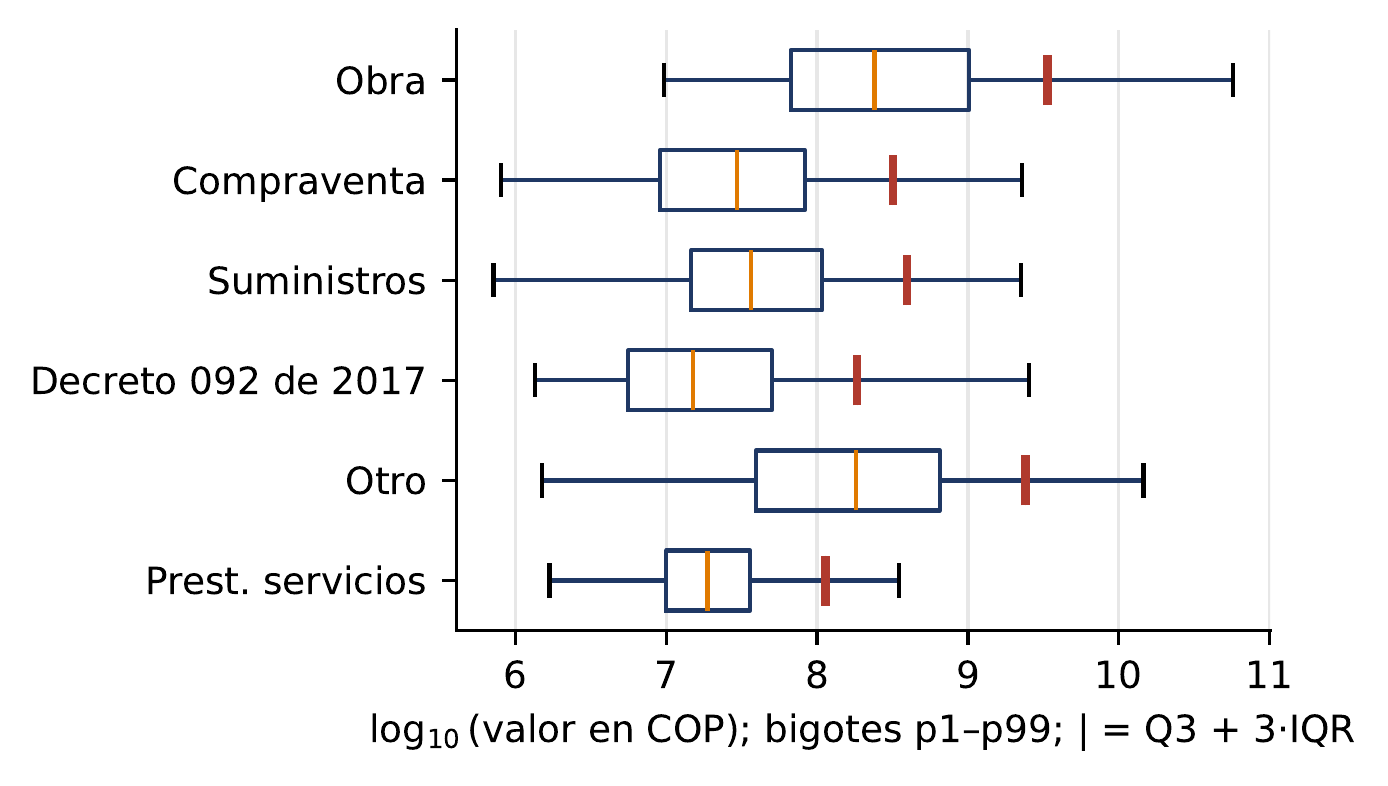
\includegraphics[width=\columnwidth]{figuras/fig_box_tipo.png}
\caption{Cómo se reparten los valores en cada tipo de contrato, sobre la muestra; la marca roja indica el límite de atípico obtenido con todos los datos.}
\label{mineria:fig:box}
\end{figure}

% =============================================================================
\subsection{Análisis exploratorio}
\label{mineria:sec:eda}
% =============================================================================
Los conteos salen exactos de las tablas de oro, y lo demás de una muestra de 51.570 contratos. La muestra se elige con un \emph{hash} del identificador, de modo que la misma consulta devuelve siempre los mismos contratos.

La contratación directa reúne el 76,6~\% de los contratos y apenas el 32,2~\% del valor, porque en su mayoría son prestaciones de servicios pequeñas, con una mediana de 18,7 millones de COP. Bogotá concentra el 32,9~\% de los contratos, y la proporción de contratación directa va del 75,7~\% allí al 90,1~\% en Valle del Cauca (Fig.~\ref{mineria:fig:departamentos}).

Se esperaba un pico en diciembre, pero cada año el mes con más contratos es enero o febrero (Fig.~\ref{mineria:fig:serie}). Los dos meses más altos de toda la serie son enero de 2022 y enero de 2026, ambos justo antes de una Ley de Garantías, y mientras dura la restricción la contratación directa pasa de más del 80~\% a menos del 20~\%. En la muestra, el 5,8~\% de los contratos se firmó en sábado o domingo y el plazo mediano es de 152 días. Fuera de la contratación directa las alertas son poco frecuentes (Tabla~\ref{adq:t7}), así que el análisis siguiente se fija en perfiles y combinaciones.

\begin{figure}[!htbp]
\centering



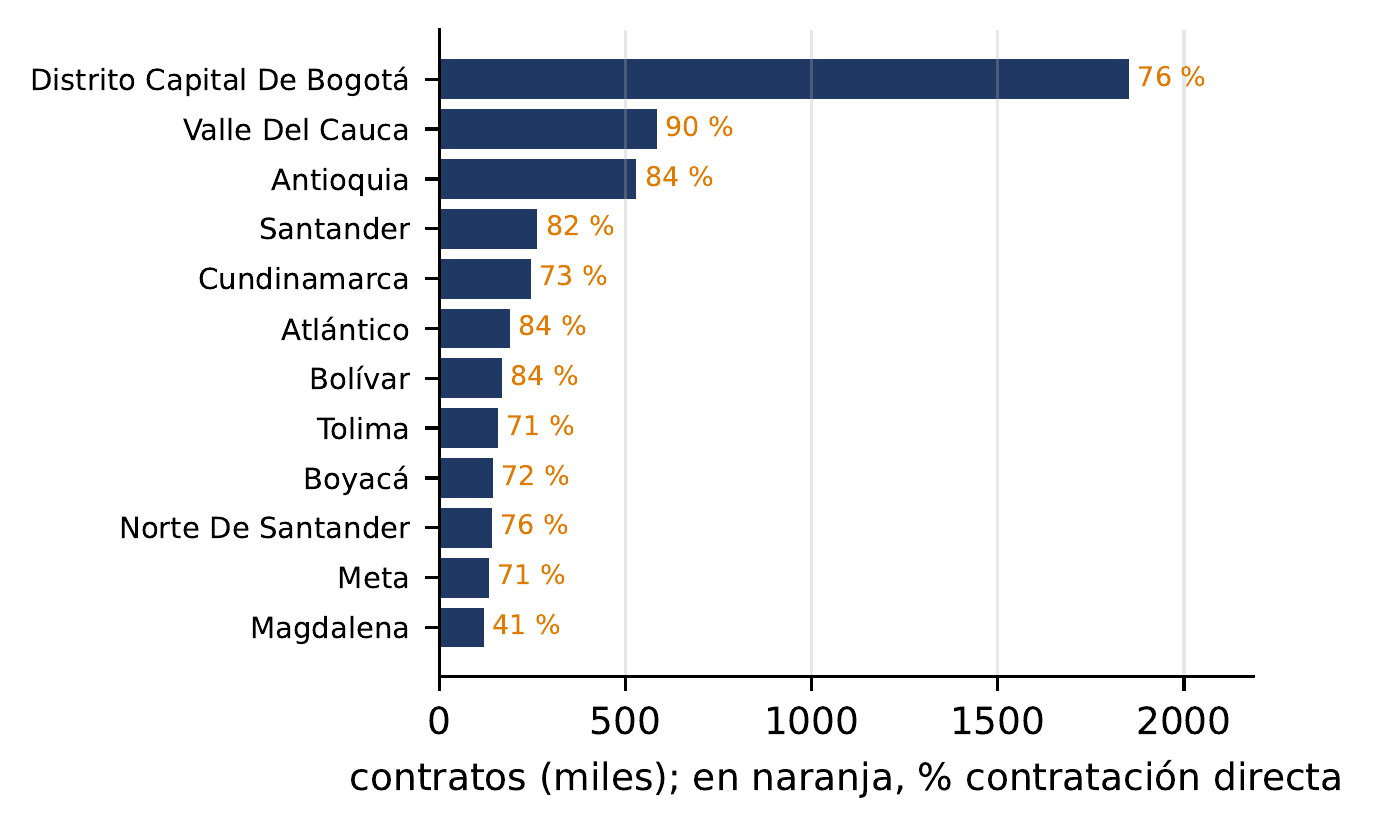
\includegraphics[width=\columnwidth]{figuras/fig_departamentos.png}
\caption{Doce departamentos con mayor número de contratos y la parte que se adjudica de forma directa.}
\label{mineria:fig:departamentos}
\end{figure}

\begin{figure}[!htbp]
\centering



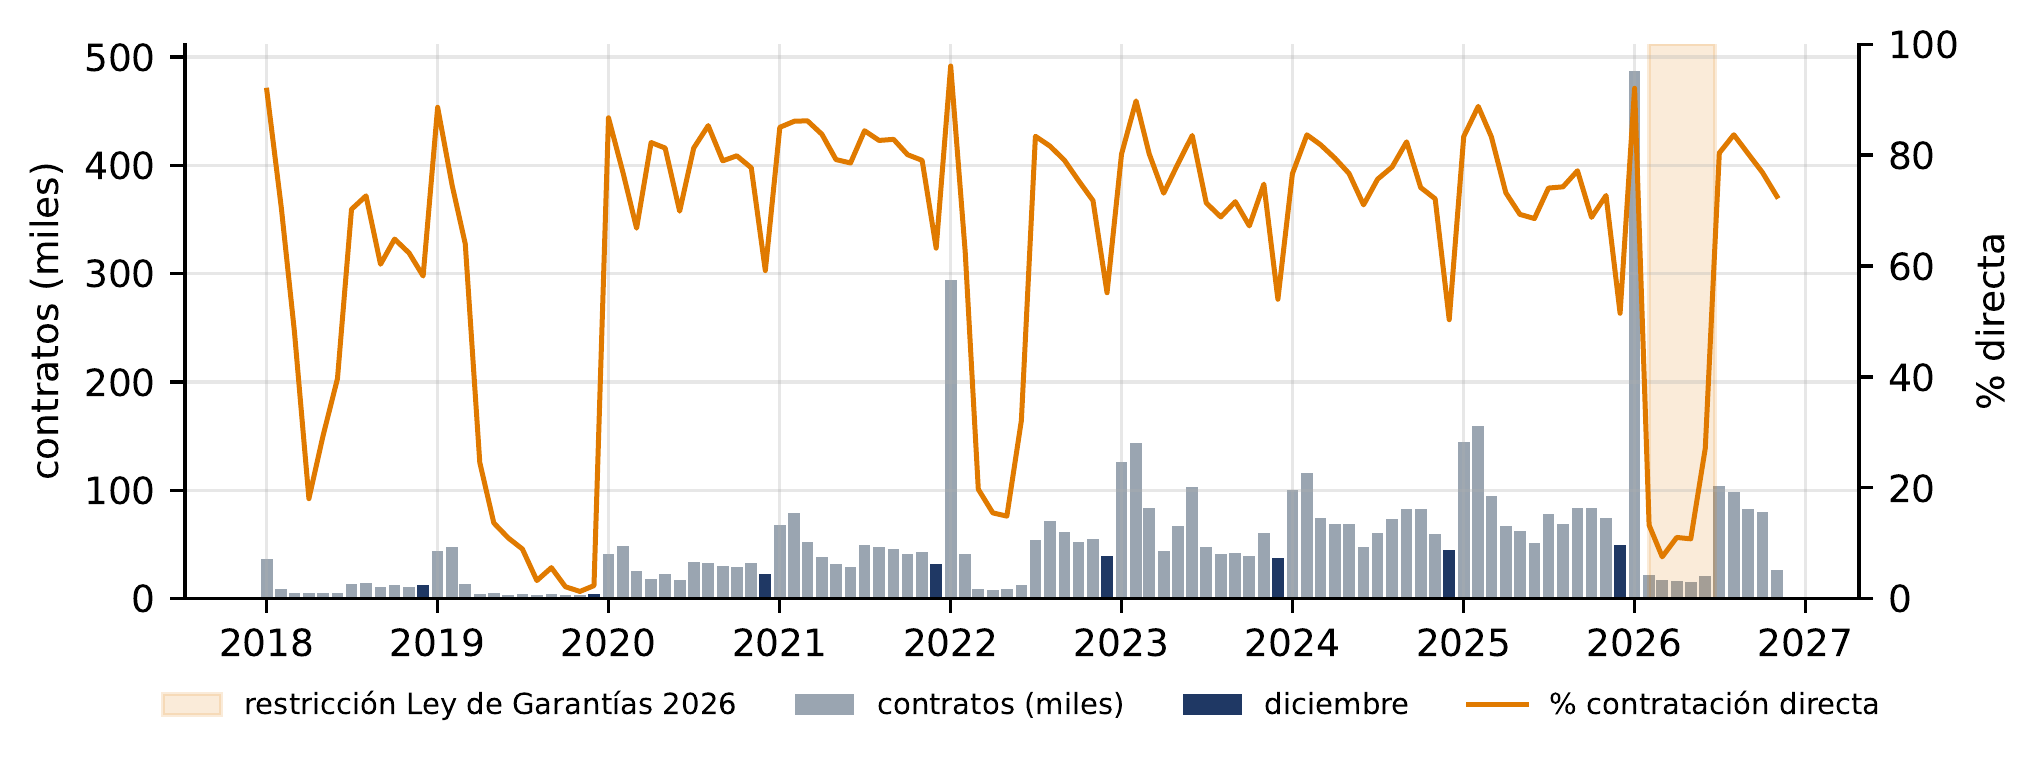
\includegraphics[width=\columnwidth]{figuras/fig_serie_mensual.png}
\caption{Contratos firmados mes a mes (barras, con diciembre destacado) y porcentaje adjudicado de forma directa (línea). En naranja, el periodo de restricción de 2026.}
\label{mineria:fig:serie}
\end{figure}

% =============================================================================
\subsection{Agrupamiento de entidades con K-means}
\label{mineria:sec:kmeans}
% =============================================================================
Se tomaron las 2.603 entidades con 20 contratos o más, que juntas suman el 99,8~\% de los contratos. Cada una se describe con ocho números: el porcentaje de sus contratos que activa cada una de siete alertas y la parte de su valor que se lleva su mayor contratista. El anticipo alto quedó fuera porque casi no varía entre entidades, y la alerta de concentración también, porque repite la participación del mayor contratista. A cada proporción se le sacó raíz cuadrada y luego se estandarizó, para que ninguna pese más que las otras en la distancia. El modelo es K-means~\cite{macqueen1967} con inicio k-means++~\cite{arthur2007}, en scikit-learn~\cite{pedregosa2011} y con semilla 42.

Para escoger $k$ se probaron valores de 2 a 10 y se compararon la inercia, la silhouette~\cite{rousseeuw1987} y el índice de Davies-Bouldin~\cite{davies1979} (Fig.~\ref{mineria:fig:codo}). De $k = 3$ en adelante, la mejor silhouette es la de $k=4$, con 0,213. Con $k=2$ los grupos solo separan a quienes contratan mucho o poco de forma directa, y eso no ayuda a priorizar. Al repetir el modelo con diez semillas, el índice de Rand ajustado~\cite{hubert1985} fue de 0,999, así que los grupos no dependen del azar. Una silhouette tan baja indica que los grupos se mezclan en los bordes y deben leerse como perfiles.

\begin{figure}[!htbp]
\centering



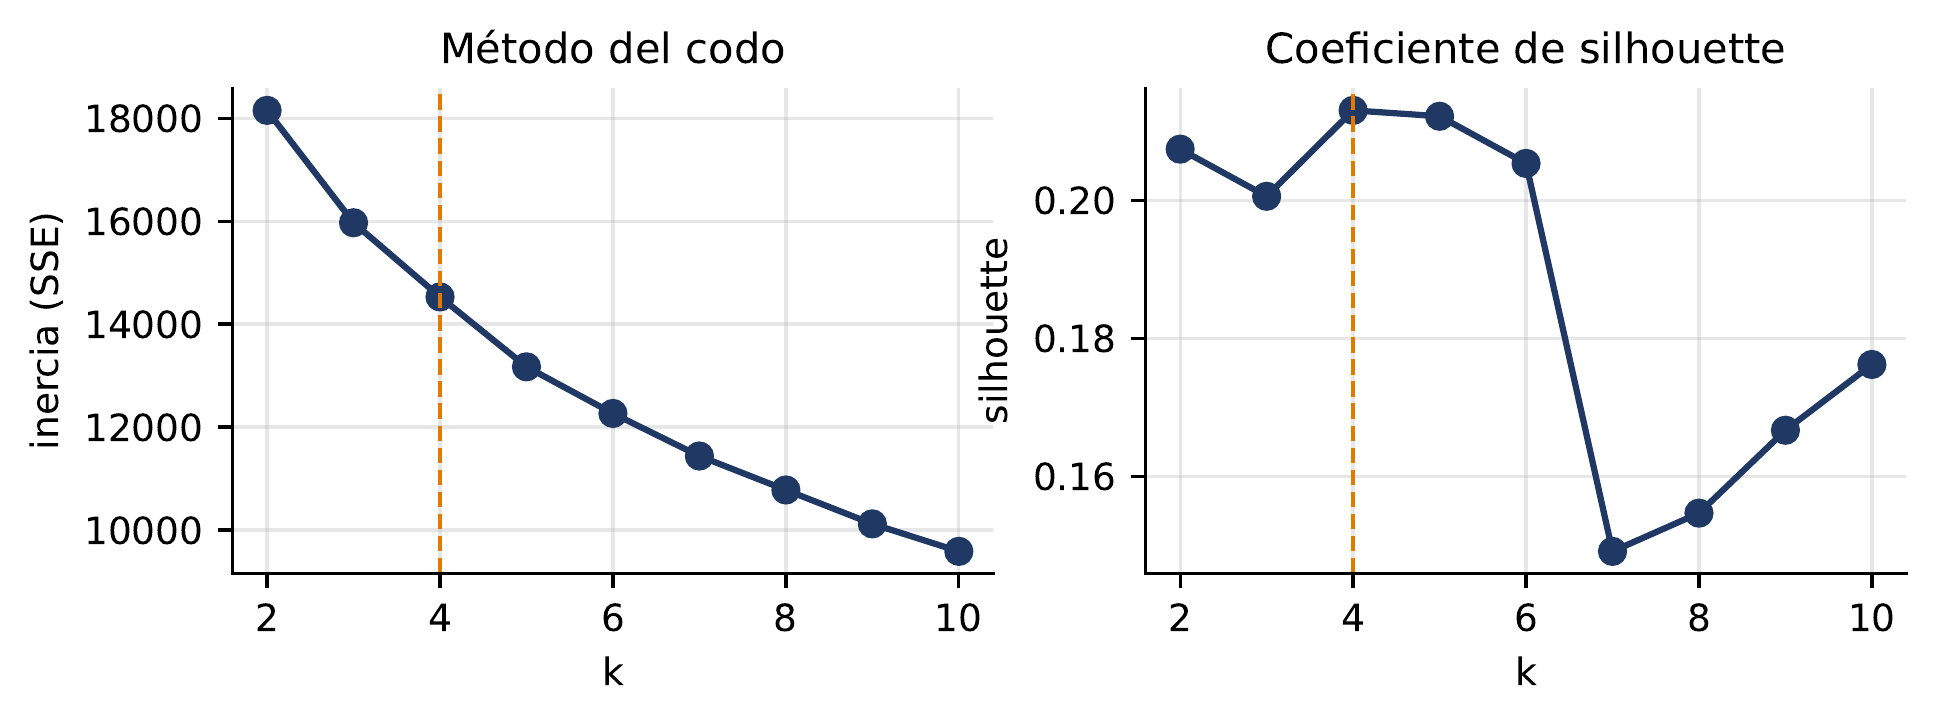
\includegraphics[width=\columnwidth]{figuras/fig_codo_silhouette.png}
\caption{Elección de $k$: inercia y silhouette. La línea naranja marca $k=4$.}
\label{mineria:fig:codo}
\end{figure}

La Fig.~\ref{mineria:fig:perfil} y la Tabla~\ref{mineria:tab:clusters} describen los cuatro grupos:
\begin{itemize}
  \item C1 reúne 541 entidades con pocas alertas y casi sin contratación directa. Muchas son hospitales públicos, que contratan por régimen especial.
  \item En las 304 entidades de C2, el 29~\% de los contratos empieza antes de firmarse, ocho veces el promedio nacional.
  \item En las 365 de C3, uno de cada cinco contratos supera el umbral de su tipo, y hay más adiciones y más contratistas sin identificar.
  \item C4 tiene 1.393 entidades que contratan de forma directa el 80,6~\% de las veces; ahí está el 77,8~\% de todos los contratos.
\end{itemize}

\begin{figure}[!htbp]
\centering



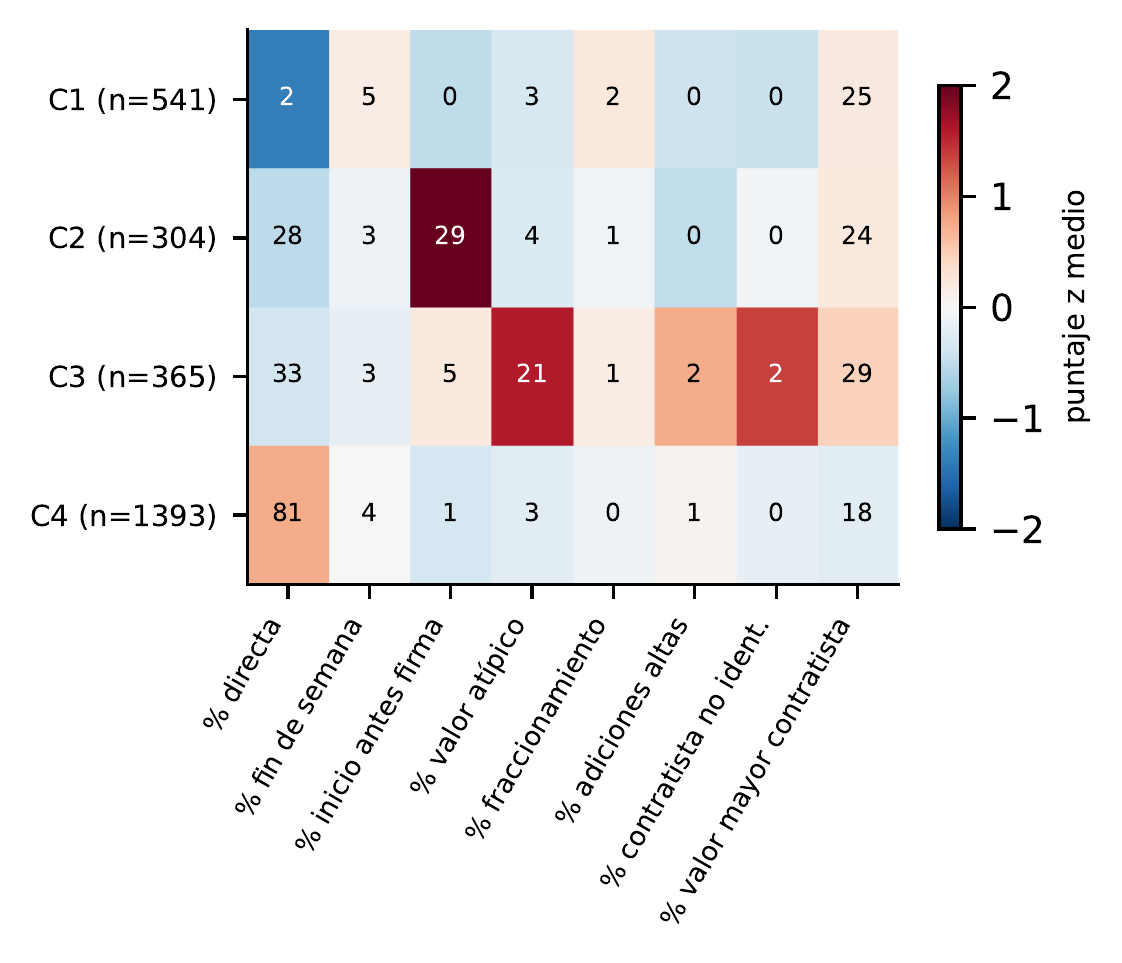
\includegraphics[width=\columnwidth]{figuras/fig_perfil_clusters.png}
\caption{Rasgos de cada grupo de entidades. El color muestra cuánto se aparta del promedio y la cifra, el porcentaje.}
\label{mineria:fig:perfil}
\end{figure}

\begin{table}[!htbp]
\centering
\caption{Promedios por entidad en cada uno de los cuatro grupos}
\label{mineria:tab:clusters}
\footnotesize
\begin{tabular}{@{}lrrrr@{}}
\toprule
 & C1 & C2 & C3 & C4 \\
\midrule
Entidades & 541 & 304 & 365 & 1.393 \\
Contratos (miles) & 381,5 & 292,3 & 590,4 & 4.426,5 \\
\% con una alerta o más & 13,5 & 55,8 & 58,9 & 83,7 \\
\% directa & 1,6 & 28,3 & 33,2 & 80,6 \\
\% inicio antes de firma & 0,3 & 29,0 & 4,8 & 0,8 \\
\% valor atípico & 3,1 & 3,5 & 21,1 & 2,6 \\
\% del principal proveedor & 24,6 & 24,3 & 29,3 & 17,8 \\
\bottomrule
\end{tabular}
\end{table}

Saber el grupo orienta la revisión: si la entidad está en C2, lo primero son las fechas; si está en C3, los montos y las prórrogas.

% =============================================================================
\subsection{Reglas de asociación entre alertas}
\label{mineria:sec:apriori}
% =============================================================================
Aquí cada contrato hace de transacción y cada alerta activa, de ítem. Athena agrupó los contratos según su combinación de alertas y encontró 129 combinaciones distintas con su número de contratos, de manera que el soporte se calcula exacto sobre todo el conjunto. Con Apriori~\cite{agrawal1994} y un soporte mínimo de 0,1~\% resultaron 21 conjuntos frecuentes y 30 reglas. La confianza y el lift de una regla $A\Rightarrow B$ son
\begin{equation}
\mathrm{conf}=\frac{\mathrm{sop}(A\cup B)}{\mathrm{sop}(A)},\qquad
\mathrm{lift}=\frac{\mathrm{conf}}{\mathrm{sop}(B)} ,
\end{equation}
y un lift por encima de 1 significa que las dos alertas coinciden más de lo que coincidirían por azar.

\begin{table}[!htbp]
\centering
\caption{Alertas que coinciden más (lift de 1,2 o más) y las que casi nunca van juntas}
\label{mineria:tab:reglas}
\footnotesize
\begin{tabular}{@{}lrrr@{}}
\toprule
Regla & Contratos & Conf. & Lift \\
\midrule
sin proveedor $\Rightarrow$ atípico & 7.170 & 44,2~\% & 10,62 \\
prórroga larga $\Rightarrow$ firmado en fin de semana & 9.846 & 14,0~\% & 2,41 \\
prórroga larga $\Rightarrow$ empezó sin firma & 6.089 & 8,7~\% & 2,36 \\
prórroga larga $\Rightarrow$ atípico & 6.251 & 8,9~\% & 2,14 \\
empezó sin firma $\Rightarrow$ atípico & 11.687 & 5,6~\% & 1,34 \\
\midrule
atípico $\Rightarrow$ adjudicación directa & 105.150 & 44,3~\% & 0,57 \\
prórroga larga $\Rightarrow$ adjudicación directa & 17.161 & 24,5~\% & 0,32 \\
\bottomrule
\end{tabular}
\end{table}

\begin{figure}[!htbp]
\centering



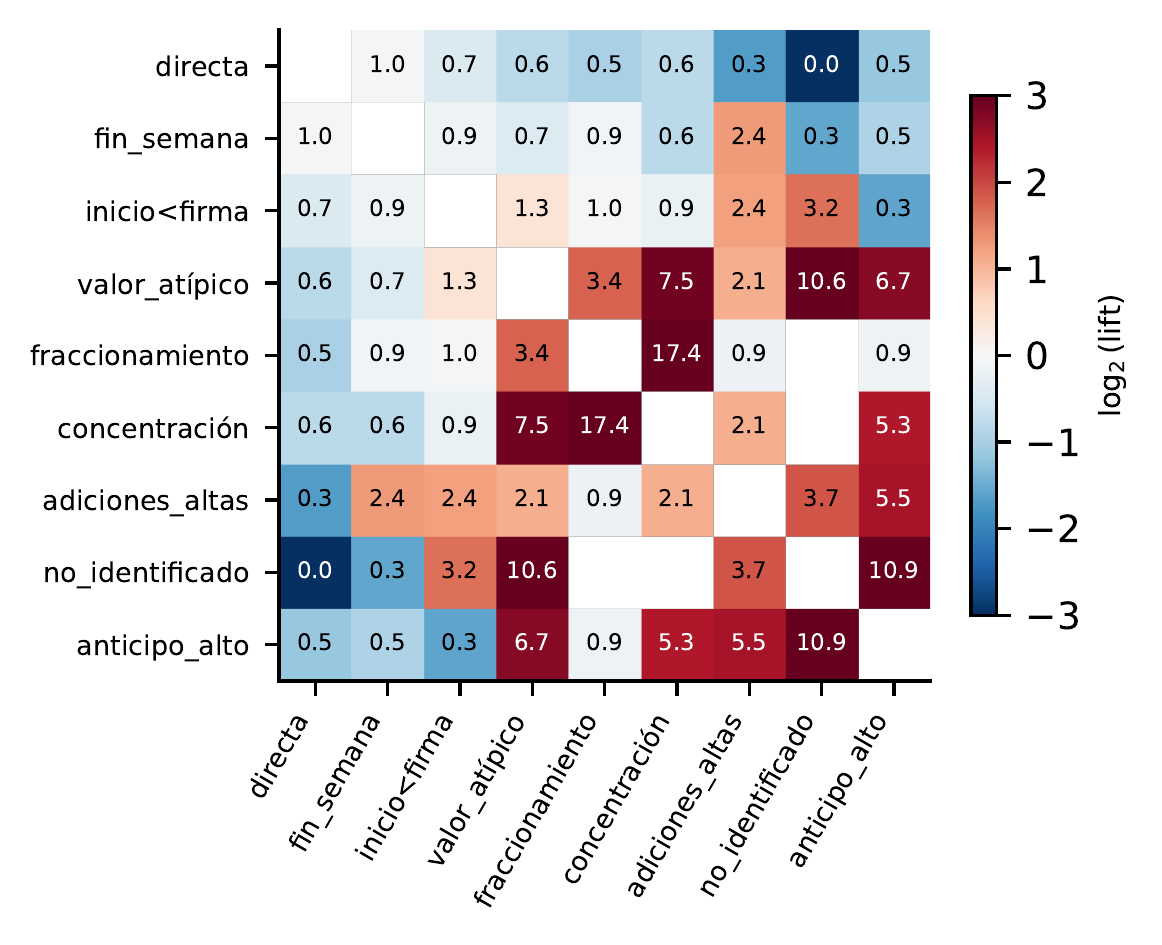
\includegraphics[width=\columnwidth]{figuras/fig_lift_pares.png}
\caption{Lift de cada par de alertas: en rojo coinciden más de lo que daría el azar y en azul, menos.}
\label{mineria:fig:lift}
\end{figure}

La relación más fuerte (Tabla~\ref{mineria:tab:reglas} y Fig.~\ref{mineria:fig:lift}) es entre no identificar al contratista y tener un valor atípico: el 44~\% de los contratos sin documento del contratista también es atípico, 10,6 veces lo esperado. Puede tratarse de contratos para revisar o de errores al publicar. Las adiciones altas suelen ir con firma en fin de semana, inicio antes de la firma y valores atípicos, lo que sugiere que los contratos mal planeados juntan varias alertas. La contratación directa, en cambio, tiene lift menor que 1 con casi todas las demás, y por eso no debería pesar tanto en el índice.

El código está en la carpeta \code{mineria/} del repositorio, con semilla fija y la misma muestra en cada corrida. Las nueve consultas leyeron 237~MB en Athena, lo que cuesta menos de un centavo de dólar~\cite{aws_athena_pricing}.

% =============================================================================
\subsection{Limitaciones}
% =============================================================================
Las alertas y los grupos señalan patrones y no dicen nada sobre la conducta de nadie, y como los grupos se mezclan en los bordes sirven para orientar la revisión, no para clasificar. Algunas entidades nacionales publican todo con un solo NIT aunque tengan sedes en varios departamentos, lo que distorsiona el análisis por territorio. Además, las cifras cambian con cada carga diaria; aquí se usa el corte del 13 de noviembre de 2026.

% =============================================================================
\subsection{Conclusiones}
% =============================================================================
\begin{itemize}
  \item Plata quedó limpia y sin duplicados, con los nulos sin rellenar y dos reglas distintas para los valores extremos.
  \item La exploración desmintió el supuesto pico de diciembre: el año arranca con la mayor contratación, en enero o febrero.
  \item K-means encontró cuatro perfiles de entidades que no cambian con la semilla, y Apriori mostró qué alertas se acompañan.
  \item Falta ponderar las alertas en el índice, probar métodos que manejen grupos mezclados, como DBSCAN o mezclas gaussianas, y revisar a mano una muestra de casos.
\end{itemize}


\finmaterias

% ===========================================================================
\section{Web de resultados}\label{sec:web}
% ===========================================================================
Para que cualquier persona use los resultados sin escribir consultas, el sistema los publica en una web:
\url{https://d48p8jbrfjaba.cloudfront.net} (Fig.~\ref{fig:web}). La web no consulta la base de datos. Al
final de cada carga semanal, una Lambda corre ocho consultas en Athena sobre la capa oro (lee unos 6~MB y
tarda menos de 20~s) y guarda los resultados como archivos JSON en un bucket privado de S3. CloudFront
entrega la página y esos archivos por HTTPS, con caché de 15 minutos, y es el único que puede leer el
bucket (Fig.~\ref{cloud:fig:arquitectura}). Como las visitas solo descargan archivos estáticos, el costo no
crece con el tráfico y cabe en la capa gratuita.

\begin{figure}[!htbp]
  \centering
  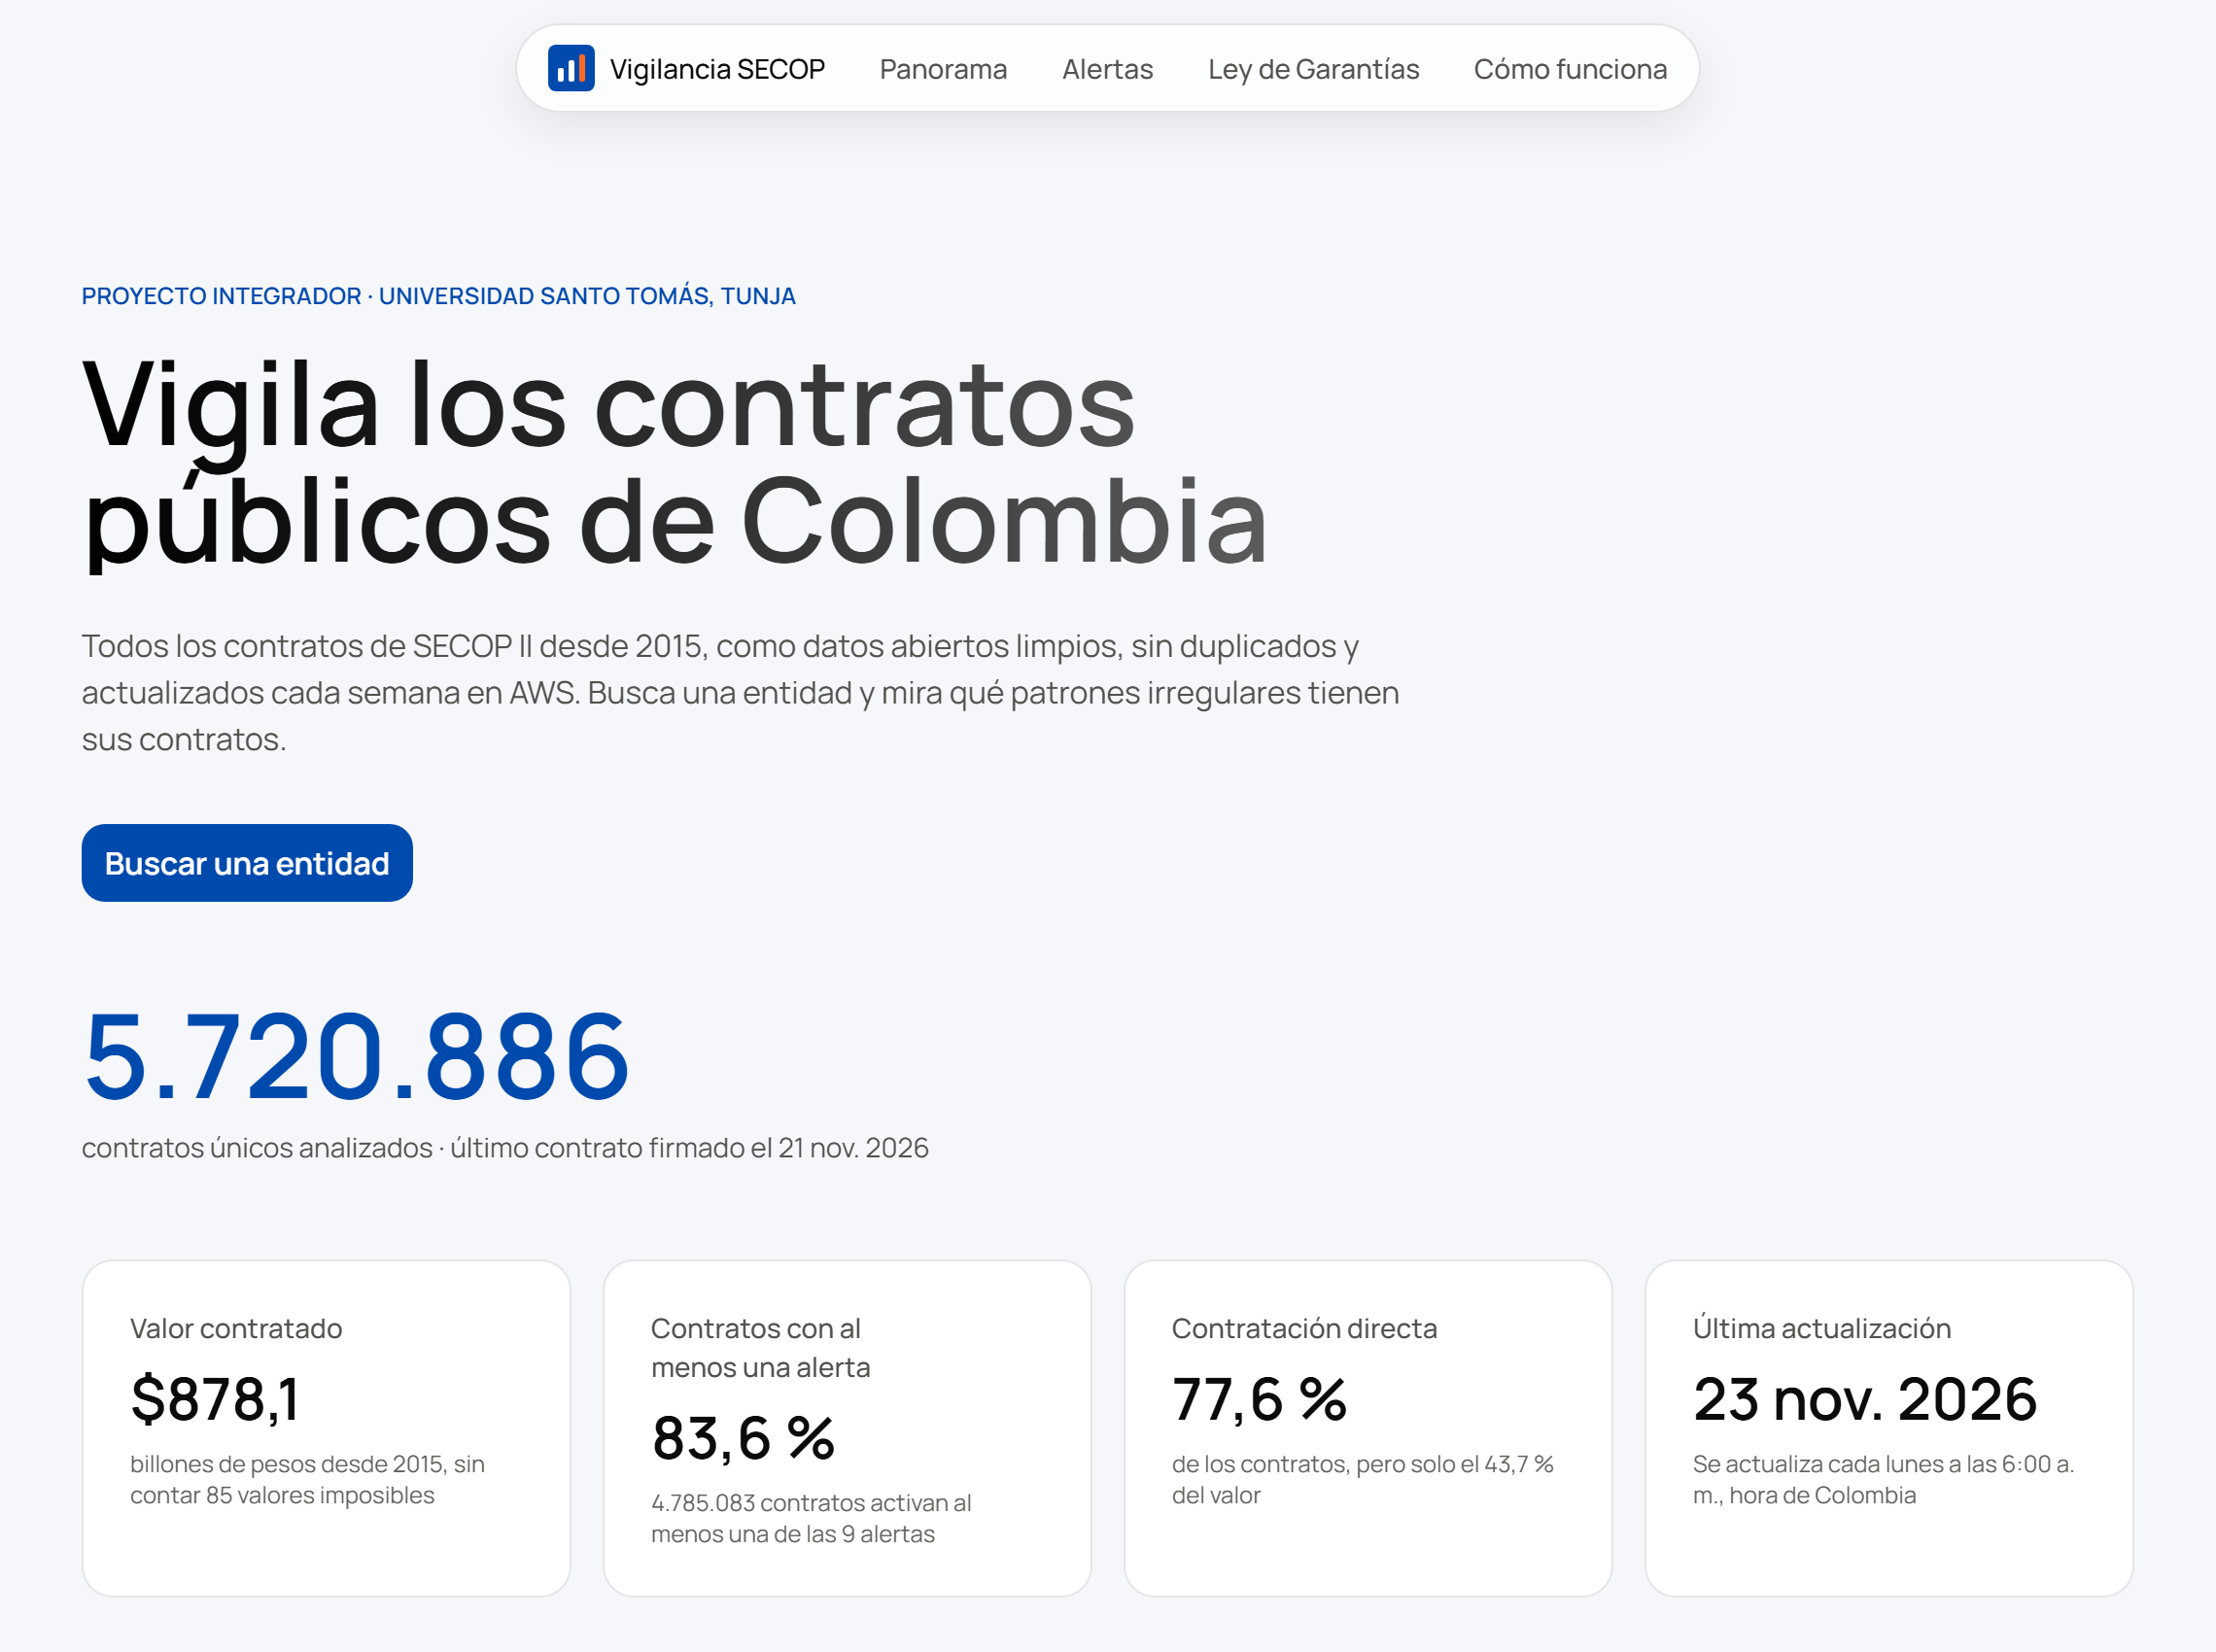
\includegraphics[width=\columnwidth]{figuras/web_resultados.png}
  \caption{Inicio de la web de resultados, con las cifras que lee de S3 (23 nov. 2026).}
  \label{fig:web}
\end{figure}

La página sigue los tres objetivos:
\begin{itemize}[leftmargin=*]
  \item \textbf{Panorama:} contratos por año, un calendario de meses y la parte que se adjudica de forma
        directa, en contratos y en valor.
  \item \textbf{Alertas:} un mapa por departamento, la frecuencia de cada alerta y un buscador de las 5.133
        entidades. La ficha de cada entidad muestra sus contratos, su valor, el porcentaje con cada alerta
        frente al promedio nacional, su puesto en el \emph{ranking} y sus contratos directos sin causal
        alrededor de la Ley de Garantías.
  \item \textbf{Ley de Garantías:} contratos directos por semana, con y sin causal de excepción, y las
        entidades con más contratos sin causal durante la restricción.
\end{itemize}
Cada gráfica tiene una tabla equivalente y se puede recorrer con el teclado.

Con los datos del 23 de noviembre de 2026 (5.720.886 contratos únicos), la web deja ver dos hechos que no
aparecían en las tablas. El mes con más contratos es enero solo en los años de elección presidencial (2018,
2022 y 2026), justo antes de la restricción de la Ley de Garantías; los demás años es febrero. Y la semana
del 26 de enero de 2026 se firmaron 141.983 contratos directos sin causal de excepción, el máximo de la
serie. La web, igual que la alerta, cuenta como directa también la modalidad «con ofertas»; por eso le da a
la contratación directa el 43,7~\% del valor, más que el 32,2~\% de la Sección~\ref{anexo:mineria}, que solo
cuenta la modalidad «Contratación directa».

El código está publicado con licencia AGPL~3.0 en
\url{https://github.com/AndresF-GaleanoT/secop-lakehouse-aws}, y los datos derivados, con la misma licencia
CC~BY-SA~4.0 de SECOP~II.

% ===========================================================================
\section{Conclusiones generales}
% ===========================================================================
El trabajo se propuso facilitar a la ciudadanía y a los entes de control la vigilancia de la contratación pública. El objetivo se cumplió:
\begin{itemize}[leftmargin=*]
  \item Los 5,69 millones de contratos de SECOP~II están en AWS: crudos en bronce (2,3~GB), limpios y sin
        duplicados en plata, y resumidos en las seis tablas de oro que responden los tres objetivos.
  \item Tres Lambdas con cuatro hilos cada una bajan el histórico en 24 minutos en vez de 44,5, y Spark procesa
        todo el histórico en unos tres minutos.
  \item El procesamiento completo costó 0,83~USD y cada actualización semanal cuesta unos 0,07~USD. Si el gasto
        llega a 15~USD en un mes, el sistema se bloquea solo.
  \item Los 85 valores imposibles quedan fuera de las sumas, pero no se borran. Con esa regla, lo
        contratado entre 2015 y 2026 suma 859 billones de COP.
  \item El 83,7~\% de los contratos activa al menos una alerta, y cuatro perfiles de entidades indican qué
        revisar en cada caso. En el mes anterior a la Ley de Garantías hubo cuatro veces más contratos
        directos sin excepción que un año antes, y durante la restricción se firmaron 4.690 sin causal
        visible.
  \item Los resultados están en una web pública que se alimenta de S3 cada semana, sin servidores y sin
        costo por visita.
\end{itemize}

Queda una tarea: montar un equipo de agentes de inteligencia
artificial capaz de revisar los archivos adjuntos a cada contrato, sean PDF u otro formato, y de detectar
incoherencias entre lo pactado, el monto, las fechas y los soportes, algo que las columnas de SECOP~II no dejan ver.

\begin{thebibliography}{99}
\small
\bibitem{ancp_secop} Agencia Nacional de Contratación Pública -- Colombia Compra Eficiente, ``SECOP~II -- Contratos Electrónicos,'' Portal de Datos Abiertos de Colombia, conjunto \texttt{jbjy-vk9h}. [En línea]. Disponible: \url{https://www.datos.gov.co/d/jbjy-vk9h}. [Accedido: 13-nov-2026].
\bibitem{ley1712} Congreso de la República de Colombia, ``Ley 1712 de 2014, por medio de la cual se crea la Ley de Transparencia y del Derecho de Acceso a la Información Pública Nacional,'' \emph{Diario Oficial}, n.\textsuperscript{o}~49.084, 6 mar. 2014.
\bibitem{ocp2016} Open Contracting Partnership, ``Red flags for integrity: Giving the green light to open data solutions,'' 2016. [En línea]. Disponible: \url{https://www.open-contracting.org/resources/red-flags-integrity-giving-green-light-open-data-solutions/}. [Accedido: 13-nov-2026].
\bibitem{fazekas2020} M. Fazekas y G. Kocsis, ``Uncovering high-level corruption: Cross-national objective corruption risk indicators using public procurement data,'' \emph{British Journal of Political Science}, vol.~50, n.\textsuperscript{o}~1, pp.~155--164, 2020, doi: 10.1017/S0007123417000461.
\bibitem{ley996} Congreso de la República de Colombia, ``Ley 996 de 2005, por medio de la cual se reglamenta la elección de Presidente de la República (Ley de Garantías Electorales),'' \emph{Diario Oficial}, n.\textsuperscript{o}~46.102, 24 nov. 2005.
\bibitem{onu_ods16} Naciones Unidas, ``Objetivo 16: Promover sociedades justas, pacíficas e inclusivas,'' Objetivos de Desarrollo Sostenible. [En línea]. Disponible: \url{https://www.un.org/sustainabledevelopment/es/peace-justice/}. [Accedido: 13-nov-2026].
\bibitem{onu_ods9} Naciones Unidas, ``Objetivo 9: Construir infraestructuras resilientes, promover la industrialización sostenible y fomentar la innovación,'' Objetivos de Desarrollo Sostenible. [En línea]. Disponible: \url{https://www.un.org/sustainabledevelopment/es/infrastructure/}. [Accedido: 13-nov-2026].
\bibitem{brown2008} T. Brown, ``Design thinking,'' \emph{Harvard Business Review}, vol.~86, n.\textsuperscript{o}~6, pp.~84--92, jun. 2008.
\bibitem{armbrust2021} M. Armbrust, A. Ghodsi, R. Xin y M. Zaharia, ``Lakehouse: A new generation of open platforms that unify data warehousing and advanced analytics,'' en \emph{Proc. 11th Conf. Innovative Data Systems Research (CIDR)}, 2021.
\bibitem{zaharia2016} M. Zaharia \emph{et al.}, ``Apache Spark: A unified engine for big data processing,'' \emph{Communications of the ACM}, vol.~59, n.\textsuperscript{o}~11, pp.~56--65, nov. 2016, doi: 10.1145/2934664.
\bibitem{tyler_soda} Tyler Technologies, ``Socrata Open Data API (SODA) documentation,'' [En línea]. Disponible: \url{https://dev.socrata.com/}. [Accedido: 13-nov-2026].
\bibitem{databricks_medallion} Databricks, ``What is the medallion lakehouse architecture?,'' [En línea]. Disponible: \url{https://docs.databricks.com/aws/en/lakehouse/medallion}. [Accedido: 13-nov-2026].
\bibitem{asf_iceberg_spec} Apache Software Foundation, ``Apache Iceberg table format specification,'' [En línea]. Disponible: \url{https://iceberg.apache.org/spec/}. [Accedido: 13-nov-2026].
\bibitem{aws_sfn_map} Amazon Web Services, ``Map workflow state,'' AWS Step Functions Developer Guide. [En línea]. Disponible: \url{https://docs.aws.amazon.com/step-functions/latest/dg/state-map.html}. [Accedido: 13-nov-2026].
\bibitem{aws_glue_guide} Amazon Web Services, ``What is AWS Glue?,'' AWS Glue Developer Guide. [En línea]. Disponible: \url{https://docs.aws.amazon.com/glue/latest/dg/what-is-glue.html}. [Accedido: 13-nov-2026].
\bibitem{ley1581} Congreso de la República de Colombia, ``Ley Estatutaria 1581 de 2012, por la cual se dictan disposiciones generales para la protección de datos personales,'' \emph{Diario Oficial}, n.\textsuperscript{o}~48.587, 18 oct. 2012.
\bibitem{ley80} Congreso de la República de Colombia, ``Ley 80 de 1993, por la cual se expide el Estatuto General de Contratación de la Administración Pública,'' \emph{Diario Oficial}, n.\textsuperscript{o}~41.094, 28 oct. 1993.
\bibitem{dean2008} J. Dean y S. Ghemawat, ``MapReduce: Simplified data processing on large clusters,'' \emph{Communications of the ACM}, vol.~51, n.\textsuperscript{o}~1, pp.~107--113, 2008, doi: 10.1145/1327452.1327492.
\bibitem{zaharia2012} M. Zaharia \emph{et al.}, ``Resilient distributed datasets: A fault-tolerant abstraction for in-memory cluster computing,'' en \emph{Proc. 9th USENIX Symp. Networked Systems Design and Implementation (NSDI)}, 2012, pp.~15--28.
\bibitem{grama2003} A. Grama, A. Gupta, G. Karypis y V. Kumar, \emph{Introduction to Parallel Computing}, 2.\textsuperscript{a} ed. Harlow, Reino Unido: Addison-Wesley, 2003.
\bibitem{psf_threading} Python Software Foundation, ``threading: Thread-based parallelism,'' The Python Standard Library. [En línea]. Disponible: \url{https://docs.python.org/3/library/threading.html}. [Accedido: 13-nov-2026].
\bibitem{psf_futures} Python Software Foundation, ``concurrent.futures: Launching parallel tasks,'' The Python Standard Library. [En línea]. Disponible: \url{https://docs.python.org/3/library/concurrent.futures.html}. [Accedido: 13-nov-2026].
\bibitem{amdahl1967} G. M. Amdahl, ``Validity of the single processor approach to achieving large scale computing capabilities,'' en \emph{Proc. AFIPS Spring Joint Computer Conf.}, 1967, pp.~483--485, doi: 10.1145/1465482.1465560.
\bibitem{gustafson1988} J. L. Gustafson, ``Reevaluating Amdahl's law,'' \emph{Communications of the ACM}, vol.~31, n.\textsuperscript{o}~5, pp.~532--533, 1988, doi: 10.1145/42411.42415.
\bibitem{karp1990} A. H. Karp y H. P. Flatt, ``Measuring parallel processor performance,'' \emph{Communications of the ACM}, vol.~33, n.\textsuperscript{o}~5, pp.~539--543, 1990, doi: 10.1145/78607.78614.
\bibitem{aws_icons} Amazon Web Services, ``AWS Architecture Icons,'' [En línea]. Disponible: \url{https://aws.amazon.com/architecture/icons/}. [Accedido: 13-nov-2026].
\bibitem{aws_lambda_quotas} Amazon Web Services, ``Lambda quotas,'' AWS Lambda Developer Guide. [En línea]. Disponible: \url{https://docs.aws.amazon.com/lambda/latest/dg/gettingstarted-limits.html}. [Accedido: 13-nov-2026].
\bibitem{tyler_order} Tyler Technologies, ``The ORDER BY clause,'' Socrata Developers. [En línea]. Disponible: \url{https://dev.socrata.com/docs/queries/order.html}. [Accedido: 13-nov-2026].
\bibitem{aws_glue_pricing} Amazon Web Services, ``AWS Glue pricing,'' [En línea]. Disponible: \url{https://aws.amazon.com/glue/pricing/}. [Accedido: 13-nov-2026].
\bibitem{aws_s3_sse} Amazon Web Services, ``Using server-side encryption with Amazon S3 managed keys (SSE-S3),'' Amazon S3 User Guide. [En línea]. Disponible: \url{https://docs.aws.amazon.com/AmazonS3/latest/userguide/UsingServerSideEncryption.html}. [Accedido: 13-nov-2026].
\bibitem{aws_iam_bp} Amazon Web Services, ``Security best practices in IAM,'' IAM User Guide. [En línea]. Disponible: \url{https://docs.aws.amazon.com/IAM/latest/UserGuide/best-practices.html}. [Accedido: 13-nov-2026].
\bibitem{aws_glue_iceberg} Amazon Web Services, ``Using the Iceberg framework in AWS Glue,'' AWS Glue Developer Guide. [En línea]. Disponible: \url{https://docs.aws.amazon.com/glue/latest/dg/aws-glue-programming-etl-format-iceberg.html}. [Accedido: 13-nov-2026].
\bibitem{aws_pricing} Amazon Web Services, ``AWS pricing,'' [En línea]. Disponible: \url{https://aws.amazon.com/pricing/}. [Accedido: 13-nov-2026].
\bibitem{aws_lambda_pricing} Amazon Web Services, ``AWS Lambda pricing,'' [En línea]. Disponible: \url{https://aws.amazon.com/lambda/pricing/}. [Accedido: 13-nov-2026].
\bibitem{aws_sfn_pricing} Amazon Web Services, ``AWS Step Functions pricing,'' [En línea]. Disponible: \url{https://aws.amazon.com/step-functions/pricing/}. [Accedido: 13-nov-2026].
\bibitem{aws_s3_pricing} Amazon Web Services, ``Amazon S3 pricing,'' [En línea]. Disponible: \url{https://aws.amazon.com/s3/pricing/}. [Accedido: 13-nov-2026].
\bibitem{aws_athena_pricing} Amazon Web Services, ``Amazon Athena pricing,'' [En línea]. Disponible: \url{https://aws.amazon.com/athena/pricing/}. [Accedido: 13-nov-2026].
\bibitem{aws_budget_actions} Amazon Web Services, ``Configuring budget actions,'' AWS Cost Management User Guide. [En línea]. Disponible: \url{https://docs.aws.amazon.com/cost-management/latest/userguide/budgets-controls.html}. [Accedido: 13-nov-2026].
\bibitem{asf_iceberg_evolution} Apache Software Foundation, ``Evolution,'' Apache Iceberg Documentation. [En línea]. Disponible: \url{https://iceberg.apache.org/docs/latest/evolution/}. [Accedido: 13-nov-2026].
\bibitem{aws_glue_versions} Amazon Web Services, ``AWS Glue versions,'' AWS Glue Developer Guide. [En línea]. Disponible: \url{https://docs.aws.amazon.com/glue/latest/dg/release-notes.html}. [Accedido: 13-nov-2026].
\bibitem{tukey1977} J. W. Tukey, \emph{Exploratory Data Analysis}. Reading, MA, EE.~UU.: Addison-Wesley, 1977.
\bibitem{macqueen1967} J. MacQueen, ``Some methods for classification and analysis of multivariate observations,'' en \emph{Proc. 5th Berkeley Symp. Mathematical Statistics and Probability}, vol.~1, 1967, pp.~281--297.
\bibitem{arthur2007} D. Arthur y S. Vassilvitskii, ``k-means++: The advantages of careful seeding,'' en \emph{Proc. 18th Annu. ACM-SIAM Symp. Discrete Algorithms (SODA)}, 2007, pp.~1027--1035.
\bibitem{pedregosa2011} F. Pedregosa \emph{et al.}, ``Scikit-learn: Machine learning in Python,'' \emph{Journal of Machine Learning Research}, vol.~12, pp.~2825--2830, 2011.
\bibitem{rousseeuw1987} P. J. Rousseeuw, ``Silhouettes: A graphical aid to the interpretation and validation of cluster analysis,'' \emph{Journal of Computational and Applied Mathematics}, vol.~20, pp.~53--65, 1987, doi: 10.1016/0377-0427(87)90125-7.
\bibitem{davies1979} D. L. Davies y D. W. Bouldin, ``A cluster separation measure,'' \emph{IEEE Trans. Pattern Anal. Mach. Intell.}, vol.~PAMI-1, n.\textsuperscript{o}~2, pp.~224--227, 1979, doi: 10.1109/TPAMI.1979.4766909.
\bibitem{hubert1985} L. Hubert y P. Arabie, ``Comparing partitions,'' \emph{Journal of Classification}, vol.~2, n.\textsuperscript{o}~1, pp.~193--218, 1985, doi: 10.1007/BF01908075.
\bibitem{agrawal1994} R. Agrawal y R. Srikant, ``Fast algorithms for mining association rules,'' en \emph{Proc. 20th Int. Conf. Very Large Data Bases (VLDB)}, 1994, pp.~487--499.
\end{thebibliography}


\end{document}
